%! suppress = Makeatletter
%! suppress = Makeatletter
\documentclass[11pt]{report}

\usepackage[T1]{fontenc}
\usepackage[utf8]{inputenc}
\usepackage{graphicx}
\usepackage{amsmath,amssymb,amsfonts}
\usepackage{polski}
\usepackage[raggedright]{titlesec}
\usepackage{indentfirst}
\usepackage{listings}
\usepackage{hyperref}
\usepackage[backend=biber, bibencoding=utf8, style=ieee, dashed=false, isbn=false, doi=false, sorting=anyvt]{biblatex}
\usepackage{caption}
\captionsetup{%
justification=raggedright,
labelfont=bf,
singlelinecheck=off
}

\addbibresource{library.bib}

\pagestyle{headings}

\renewcommand{\chaptername}{Rozdział}
\renewcommand{\contentsname}{Spis treści}
\renewcommand{\figurename}{Rys.}
\renewcommand{\tablename}{Tab.}
\renewcommand{\listfigurename}{Spis rysunków}
\renewcommand{\listtablename}{Spis tabel}
\renewcommand{\bibname}{Bibliografia}

\makeatletter
\renewcommand{\l@section}{\@dottedtocline{1}{1.5em}{2.6em}}
\renewcommand{\l@subsection}{\@dottedtocline{2}{4.0em}{3.6em}}
\renewcommand{\l@subsubsection}{\@dottedtocline{3}{7.4em}{4.5em}}
\makeatother


\begin{document}

    \begin{titlepage}
        \centering
        
\includegraphics[width=\linewidth]{fig/AGH.jpg}
        \center{\scshape WYDZIAŁ INFORMATYKI, ELEKTRONIKI\\ i~TELEKOMUNIKACJI\\
        Kierunek Informatyka}
        \vspace{0.03\textheight}
        \center{\scshape Michał Patyk}
        \bigskip
        \center{\LARGE\bfseries Analiza danych i~wzorców dotyczących wydarzeń politycznych na podstawie informacji zgromadzonych w projekcie GDELT}
        \center{(pracownia problemowa)}
        \vspace{0.2\textheight}
        \par
        \rightline{Opiekun: dr hab. inż. Koźlak Jarosław}

        \vspace{0.1\textheight}
        \center{Kraków 2020}
    \end{titlepage}

    \tableofcontents


    \chapter{Wstęp}

    W tym rozdziale została opisana motywacja oraz cele pracy.
    W części~\ref{sec:motywacja} została przedstawiona motywacja do stworzenia pracy.
    Część~\ref{sec:cele-pracy} opisuje cele pracy.
    Rozdział~\ref{ch:przegląd-dziedziny} zawiera przegląd dziedziny.
    W rozdziale~\ref{ch:koncepcja} przedstawiona została koncepcja pracy.
    Rozdział~\ref{ch:realizacja} dotyczy realizacji zadania.
    W rozdziale~\ref{ch:wstępna-analiza-danych} wykonana została wstępna analiza danych.
    Rozdział~\ref{ch:grupowanie-państw-opodobnych-cechach-orazporównanie-z-danymi-zewnętrznymi} opisuje grupowanie państw o~podobnych cechach.
    W ostatnim rozdziale~\ref{ch:podsumowanie} dokonano podsumowania przeprowadzonych analiz.
    Dodatek~\ref{ch:dodatek_niestd} zawiera szczegółowe wyniki grupowania dla danych niestandaryzowanych.
    Na końcu dokumentu dołączony został spis bibliograficzny.


    \section{Motywacja}\label{sec:motywacja}
    Projekt GDELT monitoruje doniesienia medialne ze wszystkich krajów, w ponad 100 językach, każdego dnia.
    Wszystkie wydarzenia opisane są przez aktorów, lokalizacje i~charakter aktywności, co jest specyfikowane poprzez zestaw atrybutów.
    Analiza atrybutów może umożliwić lepsze zrozumienie specyfiki krajów.
    Wykrycie wzorców może pozwolić na automatyczną reakcję na zdarzenia, prognozowanie oraz wykrywanie zdarzeń nietypowych.


    \section{Cele pracy}\label{sec:cele-pracy}
    Celem niniejszej pracy jest analiza wydarzeń politycznych oraz poszukiwanie występujących w nich wzorców w oparciu o~dane projektu GDELT.
    Zdarzenia są opisane przez aktorów.
    Wybrani zostaną aktorzy - kraje.
    Następnie kraje zostaną pogrupowane z wykorzystaniem metody k-średnich w oparciu o~wektor cech wybranych z opisu zdarzeń.
    Klastrowanie zostanie przeprowadzone przed i~po standaryzacji.
    Klastry zostaną porównane z danymi zewnętrznymi.
    Grupowanie krajów na podstawie atrybutów z bazy danych GDELT pozwoli na wykazanie związku z rzeczywistymi cechami państw.


    \chapter{Przegląd dziedziny}\label{ch:przegląd-dziedziny}
    W tym rozdziale w części~\ref{sec:gdelt} opisany został zbiór danych GDELT.
    W części~\ref{sec:cameo} przedstawiony został schemat kodowania CAMEO.
    W części~\ref{sec:przeglad} przeanalizowane zostały prace dotyczące zbioru danych GDELT.


    \section{GDELT}\label{sec:gdelt}
    GDELT - Global Database of Events, Language, and Tone - to największa, najbardziej wszechstronna i~otwarta baza danych jaka powstała.
    Wczesne poszukiwania prowadzące do stworzenia GDELT zostały opisane przez Philipa Schrodta w dokumencie~\cite{Schrodt2010} w styczniu 2010 r.
    Zbiór danych jest dostępny na stronie Projektu ~\cite{gdelt} oraz na platformie Google Cloud gdzie można z niego korzystać przez Google BigQuery~\cite{BigQuery2014}.
    GDELT używa kodowania obserwacji konfliktów i~mediacji (CAMEO)~\cite{GDELTDocumentation} do rejestrowania zdarzeń.
    W zbiorze znajdują się dane od 1979 roku.
    Kolejne porcje zdarzeń i~ich klasyfikacja generowane sa na bieżąco każdego dnia.


    \section{CAMEO}\label{sec:cameo}
    CAMEO - Conflict and Mediation Event Observations - jest schematem kodowania zdarzeń.
    Został stworzony w Katedrze Nauk Politycznych Pennsylvania State University.
    Jego początki sięgają roku 2000.
    Został zaprojektowany z myślą o~automatycznym kodowaniu i~szczegółowym kodowaniu aktorów.

    \subsection{Zdarzenia}
    Kody zdarzeń są ujednolicone pod względem kolejności numerycznej głównych kategorii.
    Kategorie są uszeregowane rosnąco względem kooperacji od 01 do 09 oraz względem konfliktu od 10 do 20.

    \subsection{Aktorzy}
    Kody aktorów składają sie z trzech znaków.
    Elementy kodu są podzielone na szerokie kategorie, takie jak podmioty państwowe, role, regiony i~grupy etniczne aktorów.


    \section{Przegląd istniejących analiz} \label{sec:przeglad}
    Zbiór danych GDELT był wielokrotnie analizowany i wykorzystywany w pracach naukowych.
    Dla słowa kluczowego GDELT multiwyszukiwarka EDS zwraca ponad 700 wyników.
    Poniżej opisanych zostanie kilka wybranych prac.

    W artykule~\cite{Yuan2017} autorzy proponują miarę siły połączenia między krajami.
    Identyfikowane są różne wzorce połączeń pomiędzy Chinami i 15 istotnymi krajami.

    W badaniu~\cite{Kwak2016} autorzy porównują zbiór danych GDELT oraz EventRegistry pod względem rozmiaru, źródeł oraz geografii wiadomości.
    GDELT okazuje się być większy zarówno pod względem ilości dokumentów jak i ilości źródeł.
    Każdy ze zbiorów posiada unikalne źródła publikujące wiele dokumentów.

    W artykule~\cite{Keertipati2014} autorzy analizują zbiór GDELT pod kątem informacji o konfliktach i pokoju.
    Badanie udowadnia, ze GDELT wychwytuje globalne trendy i pozwala na zidentyfikowanie znaczących punktów w wydarzeniach konfliktowych.
    Zaproponowany zostaje czteropoziomowy model do zaprojektowania panelu analizy zdarzeń.

    W badaniu~\cite{Ma2017} autorzy dokonują porównania tonu wypowiedzi na temat wiadomości międzynarodowych zgromadzonych w GDELT.
    Porównanie wypowiedzi z dziewięciu krajów pokazało, że mimo otrzymania różnej klasyfikacji dla wiadomości międzynarodowych w tym samym temacie, średni ton pozostaje zbliżony.

    W pracy~\cite{Wang2018} autorzy przedstawiają model metadanych dla zdarzeń politycznych.
    Na bazie tego modelu stworzono zbiór danych który został przetestowany poprzez wygenerowania raportu o wizycie prezydenta Trump'a w chinach.

    W artykule~\cite{Bodas-Sagi2016} autorzy analizują opinie na temat polityki energetycznej Hiszpanii przy użyciu GDELT.
    Stworzone wskaźniki sentymentu zostały ocenione poprzez porównanie ze zmiennymi rynku energii takimi jak cen i popyt.
    Korelacja do dziennych cen energii nie została odnaleziona.

    W badaniu~\cite{Yuan2017a} autor bada efektywność tradycyjnych modeli szeregów czasowych w przewidywaniu trendów w doniesieniach medialnych.
    Wnioskiem autora model autoregresyjny ze średnią ruchomą (ARIMA) ma ograniczone zastosowanie w określaniu międzypaństwowych relacji w odniesieniu do wielkich zbiorów danych.


    \chapter{Koncepcja}\label{ch:koncepcja}

    W tym rozdziale w części~\ref{sec:założenia-i-wymagania} zostały przedstawione założenia i~wymagania.
    W części~\ref{sec:efekt-końcowy} został opisany efekt końcowy projektu.


    \section{Założenia i~wymagania}\label{sec:założenia-i-wymagania}
    W analizie wykorzystany zostanie głównie zbiór danych GDELT 2.0 od początku 2015 roku do kwietnia 2020.
    W pierwszej kolejności zostaną przeprowadzone wstępne analizy które pozwolą lepiej zrozumieć specyfikę danych.
    Następnie zostanie przeprowadzona klasteryzacja.
    Do grupowania państw w klastry zostanie wykorzystany wektor cech z bazy GDELT oraz algorytm klastrowania k-średnich.
    Wektor będzie składał się z:
    \begin{enumerate}
        \item[•] liczby zdarzeń dla których kraj jest aktorem 1 (events),
        \item[•] liczby wzmianek (numMentions) - całkowitej liczba wzmianek o~tym wydarzeniu, we wszystkich dokumentach źródłowych podczas 15-minutowej aktualizacji, w której zostało po raz pierwszy zauważone,
        \item[•] stosunku liczby zdarzeń material conflict do material cooperation z quad description (materialConfCoop) - stosunek czterokodów z podstawowej klasyfikacji
        \item[•] stosunku liczby zdarzeń verbal conflict do verbal cooperation z quad description (verbalConfCoop) - stosunek czterokodów z podstawowej klasyfikacji
        \item[•] średniego średniego tonu (avgAvgTone) - średni „ton” wszystkich dokumentów zawierających jedną lub więcej wzmianek o~tym wydarzeniu, podczas 15-minutowej aktualizacji, w której zostało ono po raz pierwszy zauważone. Waha się od -100 (skrajnie ujemny) do +100 (skrajnie dodatni).
        \item[•] średniej miary Goldsteina (avgGoldstein) - skala Goldsteina przypisuje wynik liczbowy od -10 do +10, wychwytując teoretyczny potencjalny wpływ, jaki rodzaj zdarzenia będzie miał na stabilność kraju,
        \item[•] liczby zdarzeń Fight (fightCount)
        \item[•] liczby zdarzeń Express intent to cooperate (expressCount)
    \end{enumerate}
    Dane wykorzystane w tym doświadczeniu pochodzą ze stycznia 2020 roku.
    Przed dokonaniem klasteryzacji odrzucone zostaną wydarzenia z kodami krajów cameo niezgodnymi z kodami ISO 3166-1 alfa-3~\cite{iso_alfa3}.
    Klasteryzacja zostanie przeprowadzona dwukrotnie, za drugim razem na danych ustandaryzowanych przy pomocy modułu StandardScaler~\cite{standardScaler}.

    Dla ułatwienia interpretacji wyników grupowania zostaną dodane informacje o~PKB, wydatkach na zdrowie, zbrojenia, edukację, import oraz eksport (jako procent PKB).
    Dodatkowe dane pochodzą z bazy Banku Światowego~\cite{worldbank}, są na licencji CC BY-4.0~\cite{wblicense}, przedstawiają sytuację w 2015 roku.
    \begin{enumerate}
        \item[GDP] PKB to suma wartości dodanej brutto, w dolarach, wszystkich producentów będących rezydentami w gospodarce powiększona o~wszelkie podatki od produktów i~pomniejszona o~wszelkie dotacje nieuwzględnione w wartości produktów.
        \item[Education] Wydatki sektora instytucji rządowych i~samorządowych na edukację są wyrażone jako procent PKB.
        \item[Military] Dane dotyczące wydatków wojskowych z Międzynarodowego Instytutu Badań nad Pokojem w Sztokholmie pochodzą z definicji NATO, która obejmuje wszystkie bieżące i~kapitałowe wydatki na siły zbrojne, w tym siły pokojowe.
        Wartości mniejsze niż 0.01\% zostały odrzucone w celu dostosowania skali logarytmicznej.
        \item[Health] Poziom bieżących wydatków na zdrowie wyrażony jako procent PKB. Szacunki bieżących wydatków na zdrowie obejmują towary i~usługi zdrowotne konsumowane w każdym roku.
        \item[Import] Import towarów i~usług reprezentuje wartość wszystkich towarów i~innych usług rynkowych otrzymanych z reszty świata.
        Obejmuje wartość towarów, frachtu, ubezpieczenia, transportu, podróży, tantiem, opłat licencyjnych i~innych usług, takich jak usługi komunikacyjne, budowlane, finansowe, informacyjne, biznesowe, osobiste i~rządowe.
        Nie obejmuje kosztów związanych z zatrudnieniem i~dochodów z inwestycji oraz płatności transferowych.
        \item[Export] Eksport towarów i~usług reprezentuje wartość wszystkich towarów i~innych usług rynkowych dostarczanych do reszty świata.
    \end{enumerate}


    \section{Efekt końcowy}\label{sec:efekt-końcowy}
    Stworzony w projekcie system pozwoli na grupowanie państw na podstawie medialnych informacji zebranych w bazie GDELT.
    Przeprowadzone grupowanie państw w klastry pozwoli na uzyskanie uproszczonego, zagregowanego obrazu sytuacji geopolitycznej.
    Planowanym efektem końcowym pracy będzie wykazanie, że na bazie cech z bazy danych GDELT możemy skategoryzować państwa o~rzeczywistych cechach takich jak PKB, wydatki na zbrojenia, edukację i~ochronę zdrowia.


    \chapter{Realizacja}\label{ch:realizacja}

    W tym rozdziale w części~\ref{sec:wykorzystane-narzędzia} opisane zostały metody i~narzędzia wykorzystane podczas realizacji projektu.
    W części~\ref{sec:plan-pracy} przedstawiony został plan pracy.
    Część~\ref{sec:organizacja-pracy} prezentuje organizację pracy nad zadaniem.


    \section{Wykorzystane narzędzia}\label{sec:wykorzystane-narzędzia}

    \begin{enumerate}
        \item[•] język programowania Python~\cite{python}
        \item[•] biblioteka Pandas~\cite{pandas}
        \item[•] biblioteka GeoPandas~\cite{geopandas}
        \item[•] biblioteka Scikit-Learn~\cite{scikit}
        \item[•] środowisko programistyczne PyCharm~\cite{pycharm}
        \item[•] internetowe interaktywne środowisko obliczeniowe Notebook Jupyter~\cite{jupyter}
        \item[•] hurtownia danych Google BigQuery~\cite{bigquery}
    \end{enumerate}

    Przy tworzeniu projektu wykorzystany został język programowania Python.
    Jest to język wysokiego poziomu ogólnego przeznaczenia.
    Wraz z biblioteka Pandas jest często stosowany w zagadnieniach analizy danych oraz data miningu.
    Pandas jest łatwym w użyciu narzędziem open source które oferuje w szczególności struktury danych i~operacje do manipulacji tabelami numerycznymi.
    Głównym narzędziem używanym do programowania było zintegrowane środowisko programistyczne PyCharm firmy JetBrains.
    Pozwala ono na wygodną edycję i~analizę kodu źródłowego.
    Internetowe interaktywne środowisko obliczeniowe Notebook Jupyter pozwoliło na tworzenie dokumentów zawierających kod wraz z wizualizacjami.
    Wykorzystanie hurtowni danych Google BigQuery pozwoliło na szybką, skalowalną analizę dużego zbioru danych jakim jest GDELT.
    BigQuery jest oprogramowaniem bezserwerowym, które obsługuje zapytania w języku ANSI SQL.
    Podział krajów na klastry został wykonany przy użyciu Scikit-Learn.
    Do wizualizacji klastrów na mapie wykorzystano bibliotekę GeoPandas, która jest projektem open source mającym na celu ułatwienie pracy z danymi geograficznymi.


    \section{Plan pracy}\label{sec:plan-pracy}

    W pierwszej kolejności przeprowadzona zostanie wstępna analiza danych, która pozwoli na zorientowanie w jakim stopniu poszczególne cechy zdarzeń z bazy GDELT odzwierciedlają rzeczywiste zdarzenia i~relacje między krajami.
    Następnie przeprowadzone zostanie grupowanie państw metodą k-średnich w oparciu o~wybrane cechy zdarzeń.


    \section{Organizacja pracy}\label{sec:organizacja-pracy}
    Praca nad zadaniem przebiegała wg schematu przedstawionego na rysunku~\ref{fig:organizacjia}.

    \begin{figure}[!htp]
        \centering
        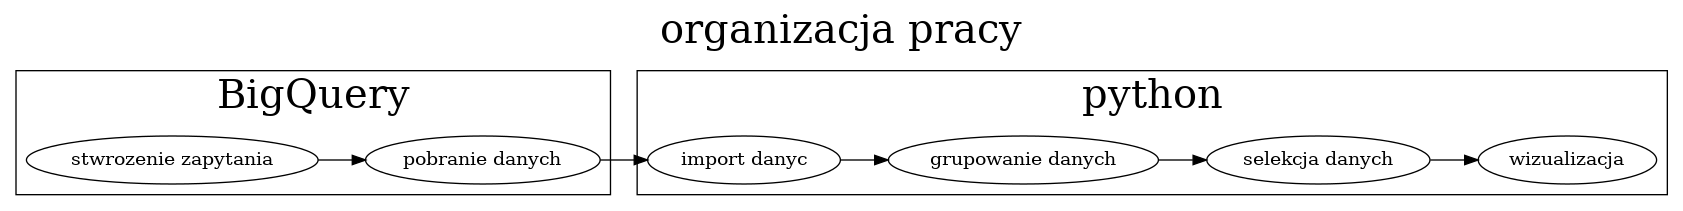
\includegraphics[width=\linewidth]{fig/organizacja.png}
        \caption{Organizacja pracy. (źródło: opracowanie własne)}
        \label{fig:organizacjia}
    \end{figure}

    Najpierw w hurtowni danych BigQuery tworzone będą zapytania do bazy danych GDELT pozwalające na agregację, filtrowanie i~grupowanie danych.
    Poniżej przykład zapytania.

    \begin{verbatim}
    SELECT
      MonthYear,
      Actor1CountryCode,
      COUNT(*) AS Events,
    FROM
      `gdelt-bq.gdeltv2.events`
    WHERE
      Year >= 2015
    GROUP BY
      MonthYear,
      Actor1CountryCode
    \end{verbatim}

    Wyniki zapytań będą zapisywane lokalnie, na dysk, do dalszej obróbki.
    Następnie w środowisku programistycznym PyCharm dla poszczególnych zagadnień tworzone będą notatniki jupyter łączące kod języka python z wizualizacjami.
    W notatnikach, zapisane wcześniej na dysku dane, będą importowane, a następnie grupowane tak aby na pojedynczym wykresie zamieści możliwie dużo informacji.
    Przedostatnim etapem będzie selekcja najistotniejszych danych w celu poprawy czytelności wykresów.
    Na końcu tworzone będą i~zapisywane do plików wizualizacje danych.

    Dane, programy oraz efekty przeprowadzonych prac można znaleźć w repozytorium \href{https://github.com/mijapa/GDELT}{GitHub}.


    \chapter{Wstępna analiza danych}\label{ch:wstępna-analiza-danych}
    W tej części pracy przeprowadzona zostanie wstępna analiza danych.
    W pierwszej kolejności w części~\ref{sec:popularność-polski-w-zbiorze-danych-gdelt} przeanalizowane zostaną dane dotyczące Polski, co pozwoli na łatwiejsze wychwycenie związków między zarejestrowanymi wydarzeniami, a sytuacją w kraju.
    W dalszej kolejności w części~\ref{sec:popularność-polski-w-zbiorze-danych-gdelt} przeprowadzona zostanie analiza wybranych krajów.
    W części~\ref{sec:analiza-siły-powiązania} przedstawiono analizę siły powiązania między wybranymi krajami.
    W części~\ref{sec:analiza-kodu-podstawowego-fight} przedstawiono analizę wybranych krajów pod kątem zdarzeń fight.


    \section{Popularność Polski w zbiorze danych GDELT}\label{sec:popularność-polski-w-zbiorze-danych-gdelt}
    Jako pierwszą analizę wykonano badanie popularności Polski w zbiorze danych GDELT. Na wszystkich trzech wykresach obserwujemy znaczny wzrost liczby zdarzeń w 2015 roku. Może być to związane z uruchomieniem w GDELT automatycznego tłumaczenia artykułów i~co za tym idzie zwiększeniem liczby źródeł danych.

    \paragraph{Polska jako Aktor 1}
    Wykres~\ref{fig:PLactor1} przedstawia popularność Polski, jako aktora 1, jako ilość zdarzeń w poszczególnych latach.
    W roku 2016 obserwujemy szczyt popularności na poziomie około 150 tysięcy zdarzeń.
    \begin{figure}[!htp]
        \centering
        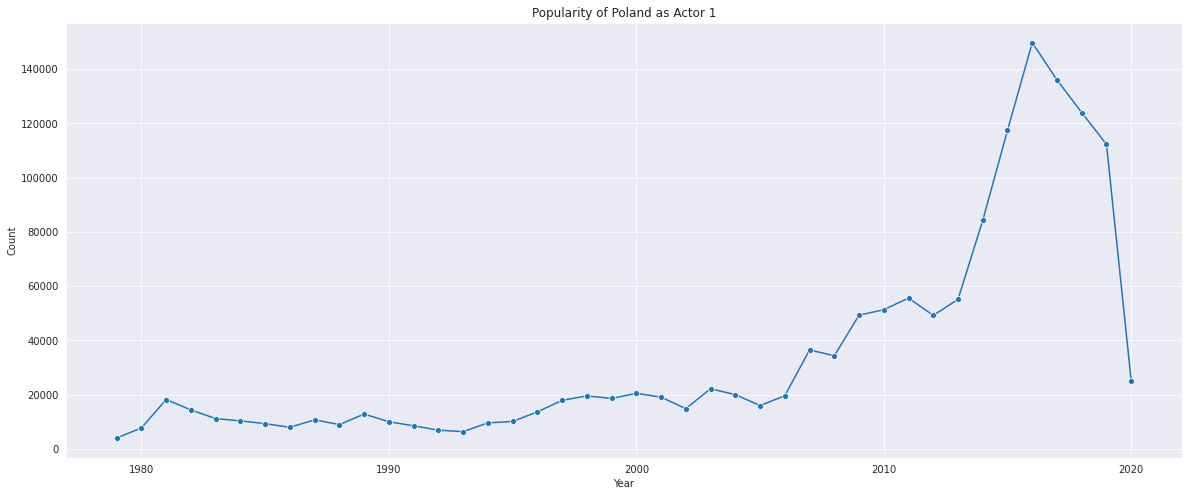
\includegraphics[width=\linewidth]{fig/PL/PLactor1.png}
        \caption{Liczba zdarzeń z Polską jako aktorem 1. (źródło: opracowanie własne)}
        \label{fig:PLactor1}
        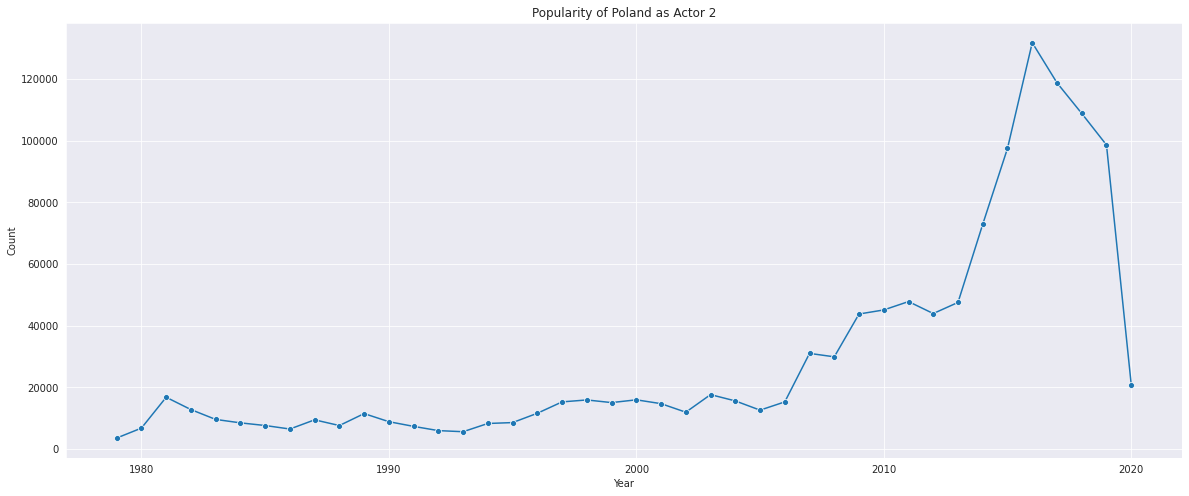
\includegraphics[width=\linewidth]{fig/PL/PLactor2.png}
        \caption{Liczba zdarzeń z Polską jako aktorem 2. (źródło: opracowanie własne)}
        \label{fig:PLactor2}
    \end{figure}

    \paragraph{Polska jako Aktor 2}
    Wykres~\ref{fig:PLactor2} przedstawia popularność Polski, jako aktora 2, jako ilość zdarzeń w poszczególnych latach.
    Kształt wykresu jest bardzo zbliżony do~\ref{fig:PLactor1} jednak szczyt popularności jest niższy - na poziomie około 130 tysięcy zdarzeń.

    \paragraph{Polska jako miejsce wydarzeń}
    Wykres~\ref{fig:PLlocation} przedstawia popularność Polski jako miejsca wydarzeń w poszczególnych latach.
    Ponownie kształt wykresu jest zbliżony do~\ref{fig:PLactor1}.
    W tym przypadku szczyt popularności jest wyższy - na poziomie około 210 tysięcy zdarzeń.

    \begin{figure}[!htp]
        \centering
        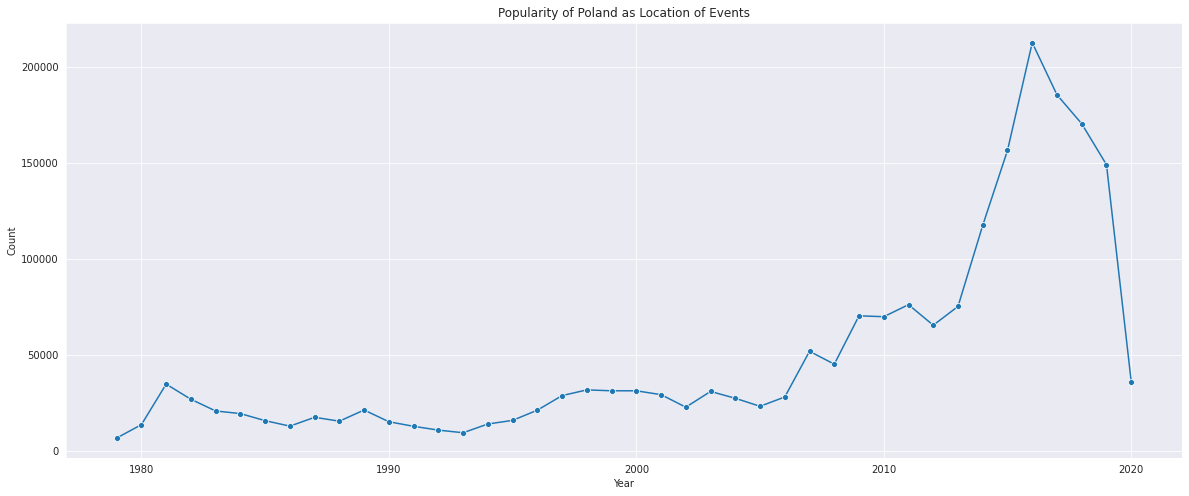
\includegraphics[width=\linewidth]{fig/PL/PLlocation.png}
        \caption{Liczba zdarzeń z Polską jako lokacją. (źródło: opracowanie własne)}
        \label{fig:PLlocation}
    \end{figure}

    \subsection{Analiza zbiorcza od 2015 roku}
    Dane pochodzą z przedziału od stycznia 2015 do kwietnia 2020 roku.

    \paragraph{Liczba zdarzeń dla poszczególnych krajów}
    Wykres~\ref{fig:GLOBALactor1} przedstawia sumaryczną liczbę zdarzeń od 2015 roku, dla poszczególnych krajów, uszeregowaną malejąco.
    \begin{figure}[!htp]
        \centering
        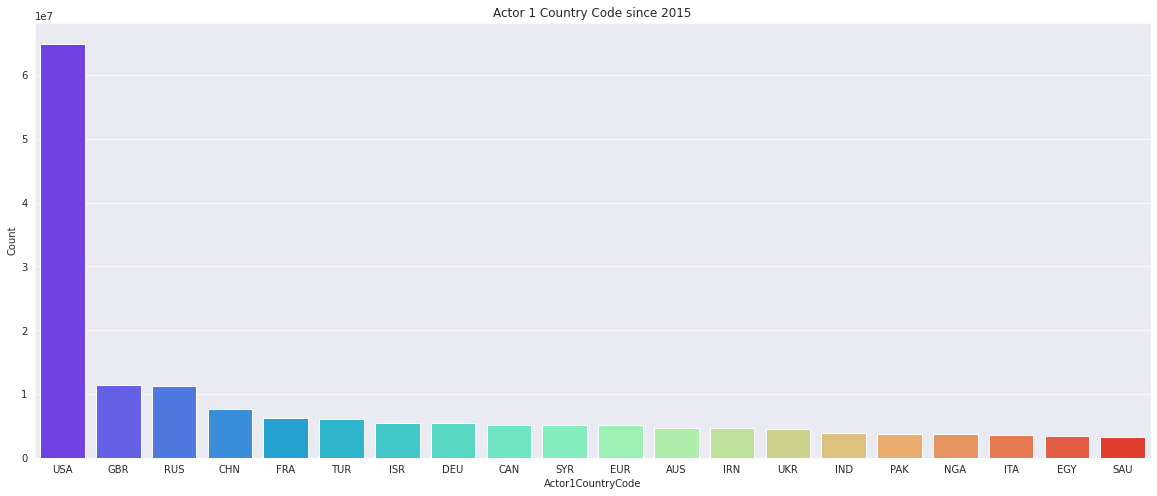
\includegraphics[width=\linewidth]{fig/GLOBAL/Actor1.png}
        \caption{Liczba zdarzeń dla poszczególnych krajów od 2015 roku. (źródło: opracowanie własne)}
        \label{fig:GLOBALactor1}
    \end{figure}
    Niekwestionowanym liderem pod względem liczby zdarzeń są Stany Zjednoczone. Dystansują one pozostałe kraje o~prawie rząd wielkości.
    Kraje anglosaskie są szczególnie mocno reprezentowane.
    W czołówce pojawiają sie też kraje znaczące politycznie oraz silnie skonfliktowane.

    \paragraph{Liczba zdarzeń w czasie}
    Wykres~\ref{fig:GLOBALactor1inTime} przedstawia liczbę zdarzeń dla top 10 krajów w poszczególnych latach (z pominięciem USA).
    \begin{figure}[!htp]
        \centering
        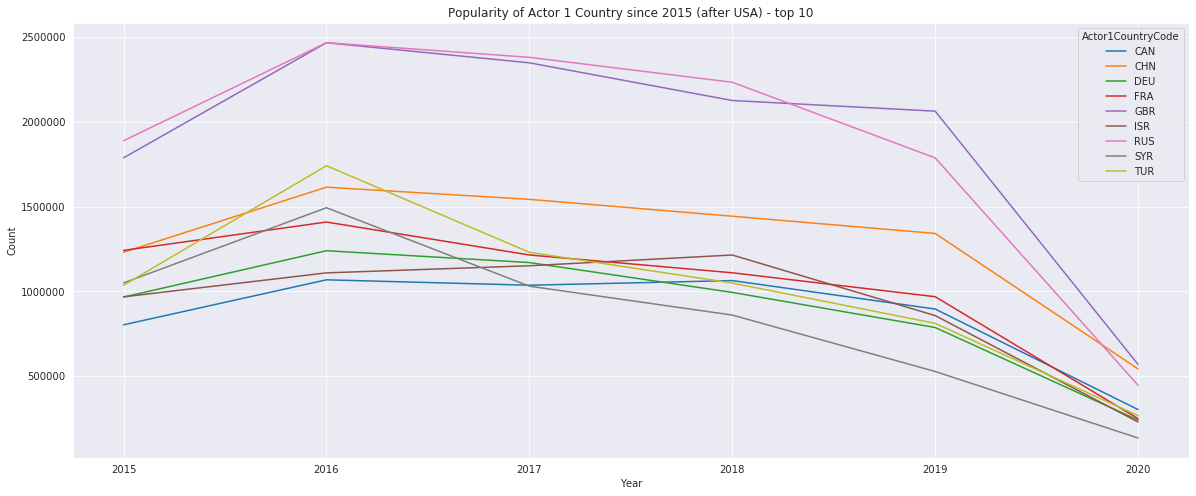
\includegraphics[width=\linewidth]{fig/GLOBAL/Actor1inTIMEafterUSA.png}
        \caption{Liczba zdarzeń dla poszczególnych krajów w czasie - top 10. (źródło: opracowanie własne)}
        \label{fig:GLOBALactor1inTime}
    \end{figure}
    Dla większości krajów szczyt ilości zdarzeń przypada na rok 2016.
    Wyraźna przewagę nad innymi krajami mają Rosja oraz Wielka Brytania.

    \paragraph{Popularność czterokodów zdarzeń}
    Wykres~\ref{fig:GLOBALQC} przedstawia sumaryczną liczbę zdarzeń od 2015 roku, dla poszczególnych czterokodów zdarzeń, uszeregowaną malejąco.
    \begin{figure}[!htp]
        \centering
        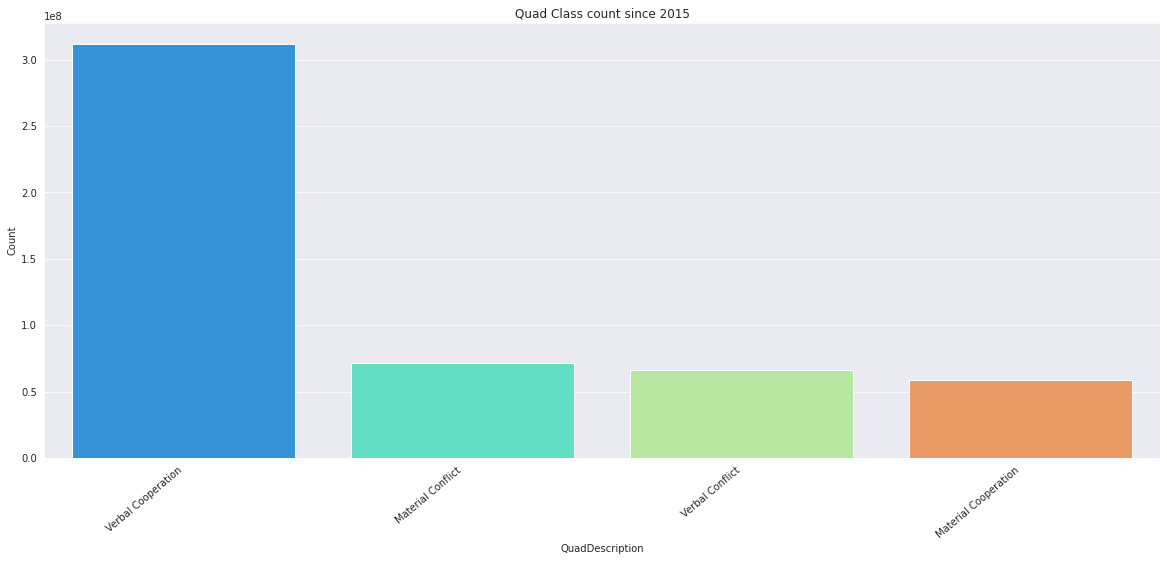
\includegraphics[width=\linewidth]{fig/GLOBAL/QC.png}
        \caption{Liczba zdarzeń dla poszczególnych czterokodów w czasie. (źródło: opracowanie własne)}
        \label{fig:GLOBALQC}
    \end{figure}
    Obserwujemy podobną tendencję jak na wykresie~\ref{fig:GLOBALactor1inTime}.
    Szczyt ilości zdarzeń przypada na rok 2016.
    Następnie ilość zdarzeń dla wszystkich czterokodów wyraźnie maleje.
    Największa ilość zdarzeń przypada kodowi \textit{verbal cooperation}.

    \paragraph{Popularność czterokodów zdarzeń w czasie}
    Wykres~\ref{fig:GLOBALQCperc} przedstawia procentową liczbę zdarzeń dla czterokodów w poszczególnych latach.
    \begin{figure}[!htp]
        \centering
        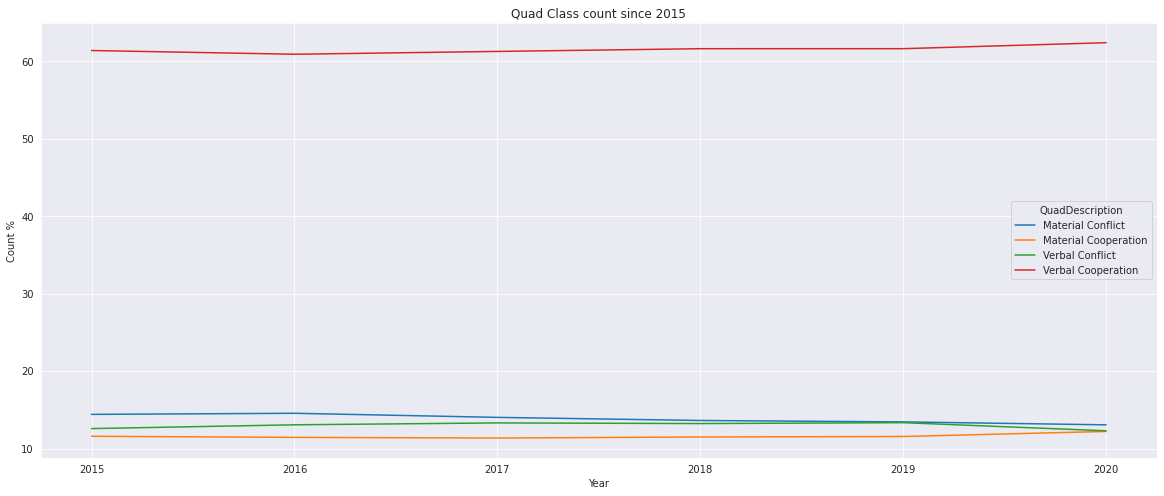
\includegraphics[width=\linewidth]{fig/GLOBAL/QCperc.png}
        \caption{Procentowa liczba zdarzeń dla poszczególnych kodów w czasie. (źródło: opracowanie własne)}
        \label{fig:GLOBALQCperc}
    \end{figure}
    Pomimo spadku ilości zdarzeń obserwowanego na wykresie~\ref{fig:GLOBALQC} procentowa ilość czterokodów w ciągu lat pozostaje na podobnym poziomie.
    Podobnie jak na poprzednim wykresie - największa ilość zdarzeń przypada kodowi \textit{verbal cooperation}.

    \paragraph{Popularność podstawowych kodów zdarzeń}
    Wykres~\ref{fig:GLOBALERC} przedstawia sumaryczną liczbę zdarzeń od 2015 roku, dla wszystkich podstawowych kodów zdarzeń, uszeregowaną malejąco.
    \begin{figure}[!htp]
        \centering
        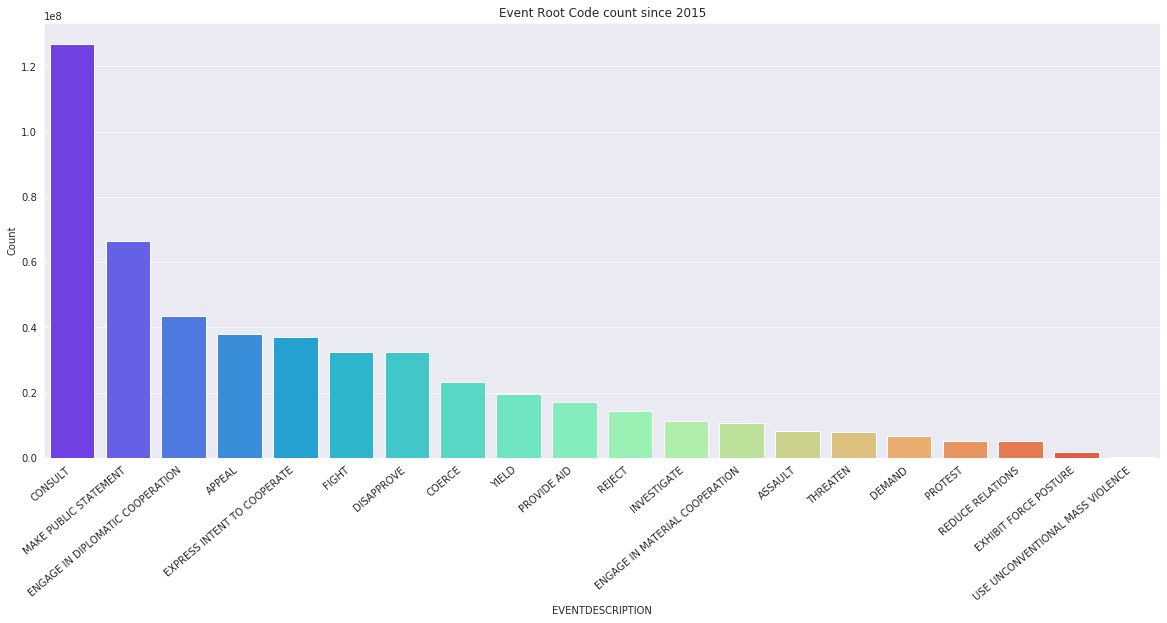
\includegraphics[width=\linewidth]{fig/GLOBAL/ERC.png}
        \caption{Liczba zdarzeń dla poszczególnych kodów podstawowych od 2015 roku. (źródło: opracowanie własne)}
        \label{fig:GLOBALERC}
    \end{figure}
    Obserwujemy prawie dwukrotną przewagę kodu \textit{CONSULT} nad następnym w kolejności kodem \textit{MAKE PUBLIC STATEMENT}.

    \paragraph{Popularność podstawowych kodów zdarzeń w czasie}
    Wykres~\ref{fig:GLOBALERCperc} przedstawia liczbę zdarzeń dla top 20 podstawowych kodów zdarzeń w poszczególnych latach.
    \begin{figure}[!htp]
        \centering
        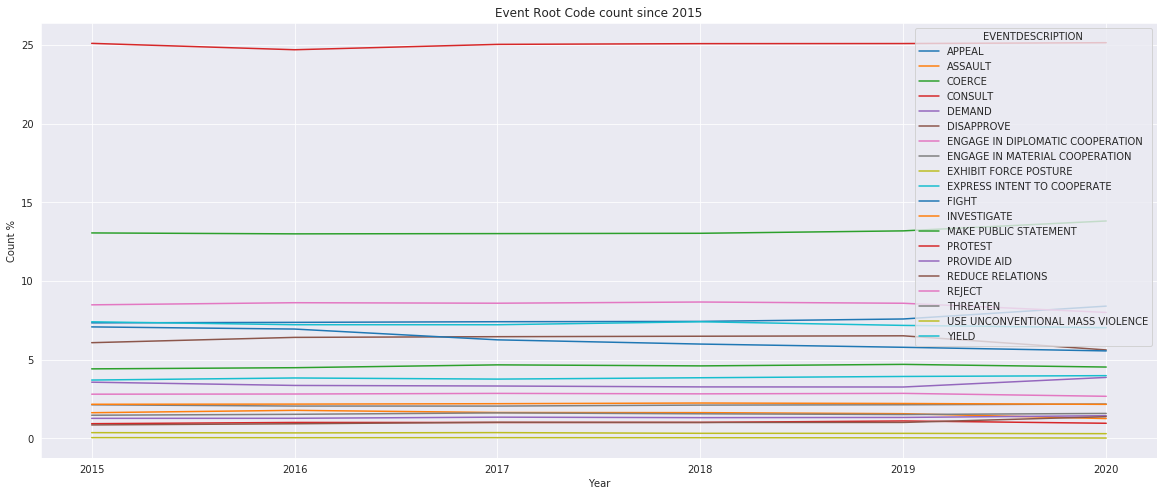
\includegraphics[width=\linewidth]{fig/GLOBAL/ERCperc.png}
        \caption{Procentowa liczba zdarzeń dla poszczególnych kodów podstawowych w czasie. (źródło: opracowanie własne)}
        \label{fig:GLOBALERCperc}
    \end{figure}
    Procentowo liczba zdarzeń dla poszczególnych kodów podstawowych utrzymuje sie na tym samym poziomie.
    Pierwsze trzy kody podstawowe to: \textit{CONSULT, COERCE} oraz \textit{ENGAGE IN DIPLOMATIC COOPERATION}.

    \paragraph{Popularność bazowych kodów zdarzeń}
    Wykres~\ref{fig:GLOBALEBC} przedstawia sumaryczną liczbę zdarzeń od 2015 roku, dla poszczególnych bazowych kodów zdarzeń, uszeregowaną malejąco.
    \begin{figure}[!htp]
        \centering
        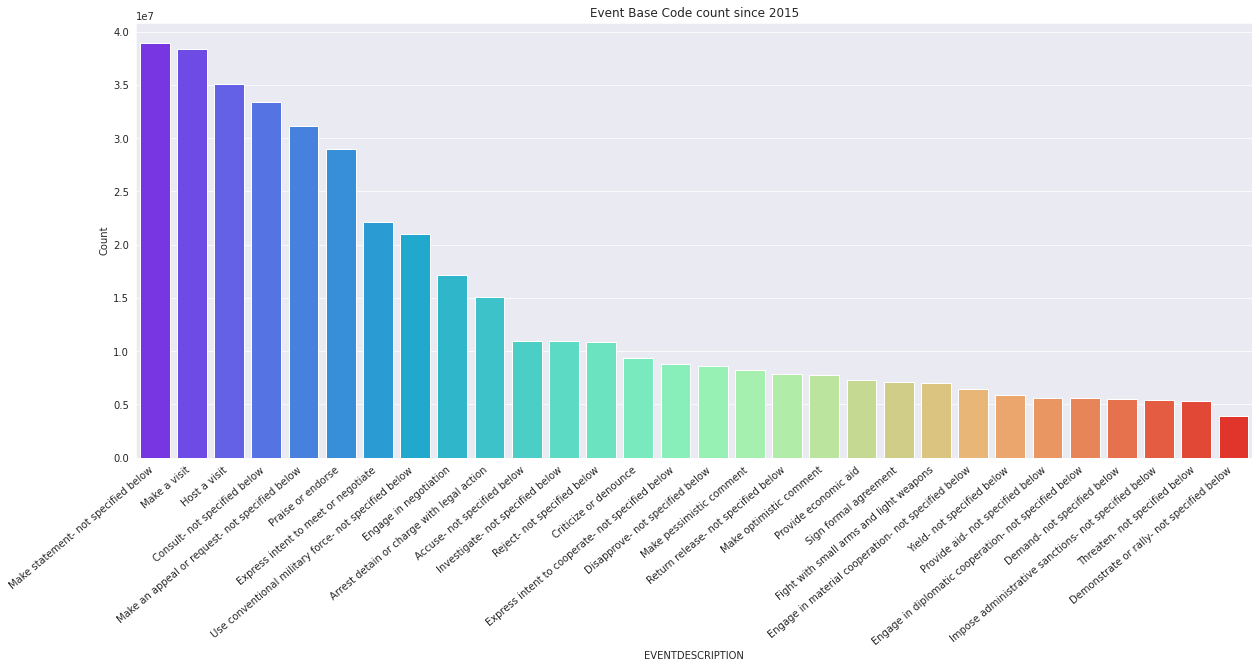
\includegraphics[width=\linewidth]{fig/GLOBAL/EBC.png}
        \caption{Liczba zdarzeń dla poszczególnych kodów bazowych od 2015 roku - top 30. (źródło: opracowanie własne)}
        \label{fig:GLOBALEBC}
    \end{figure}
    Największa ilość zdarzeń przypada dla kodów \textit{Make statement- not specified below} oraz \textit{Make a visit, Host a visit}.

    \paragraph{Procentowa popularność bazowych kodów zdarzeń w czasie}
    Wykres~\ref{fig:GLOBALEBCperc} przedstawia procentową liczbę zdarzeń dla top 10 bazowych kodów zdarzeń w poszczególnych latach.
    \begin{figure}[!htp]
        \centering
        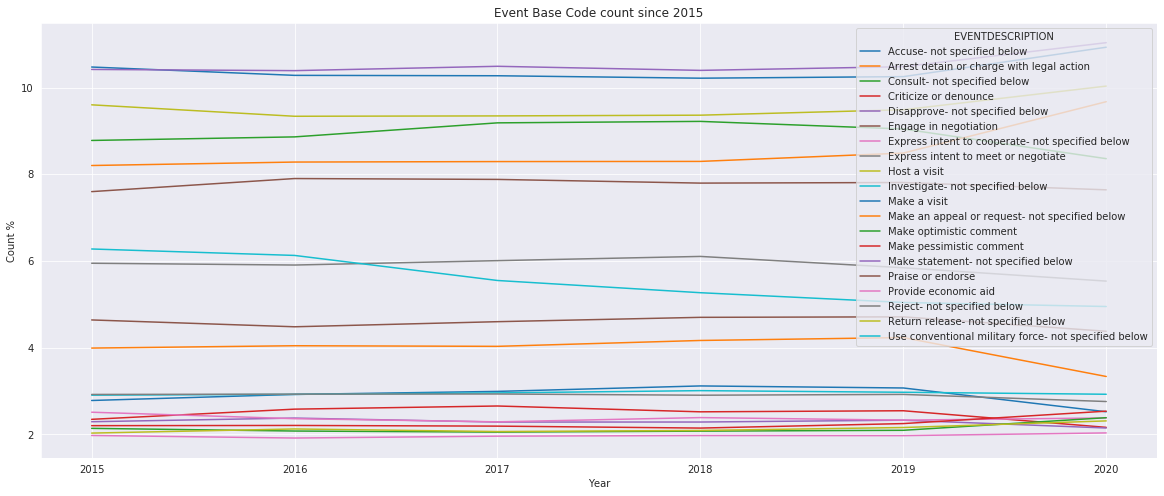
\includegraphics[width=\linewidth]{fig/GLOBAL/EBCperc.png}
        \caption{Procentowa liczba zdarzeń dla poszczególnych kodów bazowych w czasie - top 10. (źródło: opracowanie własne)}
        \label{fig:GLOBALEBCperc}
    \end{figure}
    W kolejnych latach procentowa liczba zdarzeń dla kodów bazowych zmienia sie tylko nieznacznie.
    Wyraźną zmianą jest spadek popularności kodu \textit{Use conventional military force- not specified below} w kolejnych latach.


    \section{Analiza danych dla wybranych krajów}\label{sec:analiza-danych-dla-wybranych-krajów}

    \subsection{Polska}

    \paragraph{Kraj para do zdarzenia}


    Wykres~\ref{fig:PLpair} przedstawia liczbę zdarzeń dla Polski w których parą jest dany kraj od 2015 roku.

    \begin{figure}[!htp]
        \centering
        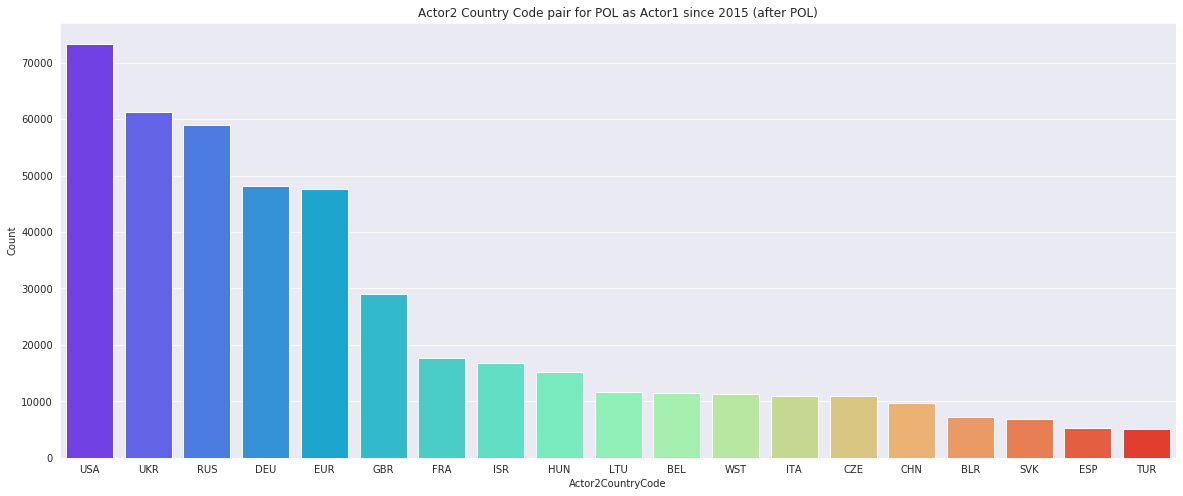
\includegraphics[width=\linewidth]{fig/PL/PLactor2Pair.png}
        \caption{Liczba zdarzeń dla Polski w których parą jest dany kraj od 2015 roku. (źródło: opracowanie własne)}
        \label{fig:PLpair}
    \end{figure}
    Najbardziej popularną parą w zdarzeniach dla Polski jest ona sama.
    Kolejnymi wg popularności krajami są Stany Zjednoczone Ameryki, Ukraina oraz Rosja.

    Wykres~\ref{fig:PLpairPerc} przedstawia liczbę zdarzeń dla Polski w których parą jest dany kraj w czasie.
    \begin{figure}[!htp]
        \centering
        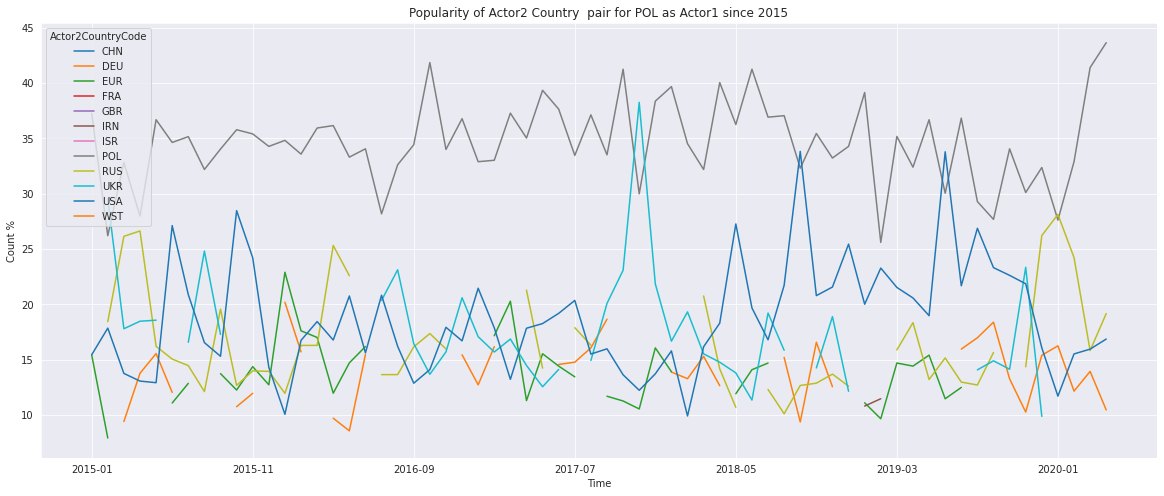
\includegraphics[width=\linewidth]{fig/PL/PLactor2PairPercinTIME.png}
        \caption{Procentowa liczba zdarzeń dla Polski w których parą jest dany kraj w kolejnych miesiącach. (źródło: opracowanie własne)}
        \label{fig:PLpairPerc}
    \end{figure}
    Tylko w czterech miesiącach Polska nie jest główną parą zdarzeń dla samej siebie.
    Dwa razy wyprzedza ją Ukraina, raz Stany Zjednoczone Ameryki, raz Rosja.
    Począwszy od sierpnia 2017 do lutego 2018 roku obserwujemy dużą ilość zdarzeń z Ukrainą.
    Następnie pierwszeństwo przejmują Stany Zjednoczone, a od listopada 2019 roku Rosja.

    \paragraph{Podstawowy kod zdarzeń}

    Wykres~\ref{fig:PLPERC} przedstawia liczbę zdarzeń z Polską dla poszczególnych kodów podstawowych od 2015 roku.
    \begin{figure}[!htp]
        \centering
        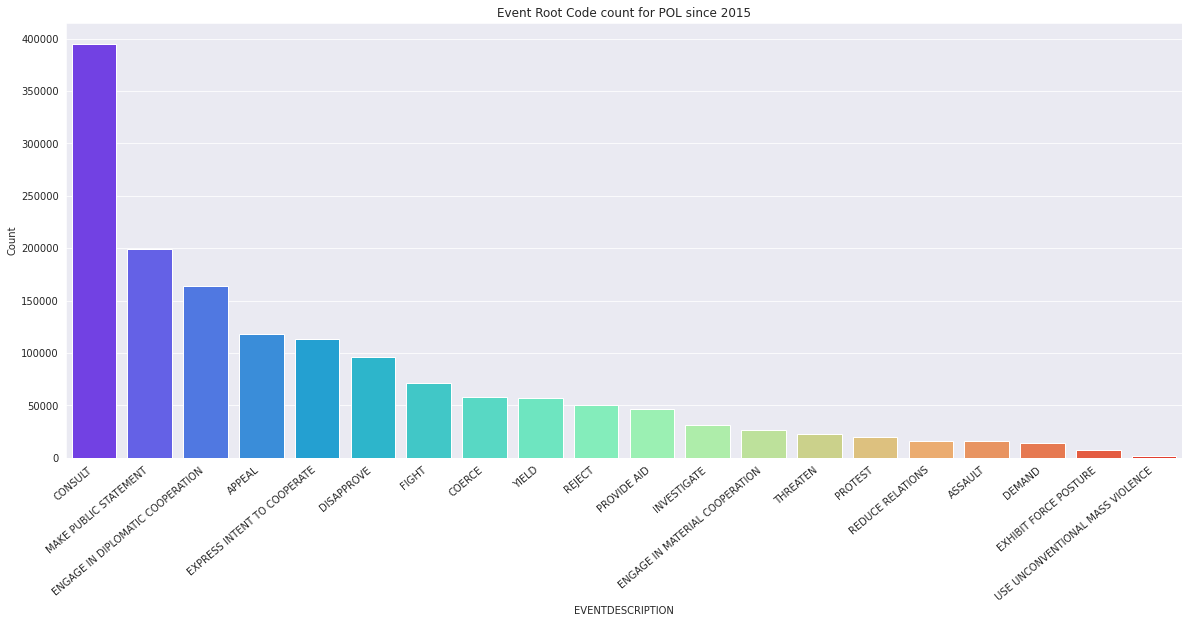
\includegraphics[width=\linewidth]{fig/PL/PLERC.png}
        \caption{Liczba zdarzeń z Polską dla poszczególnych kodów podstawowych od 2015 roku. (źródło: opracowanie własne)}
        \label{fig:PLPERC}
    \end{figure}
    Obserwujemy prawie dwukrotną przewagę kodu \textit{CONSULT} nad następnym w kolejności kodem \textit{MAKE PUBLIC STATEMENT}.

    Wykres~\ref{fig:PLPERCinTIME} przedstawia liczbę zdarzeń dla Polski dla poszczególnych kodów podstawowych w czasie.
    \begin{figure}[!htp]
        \centering
        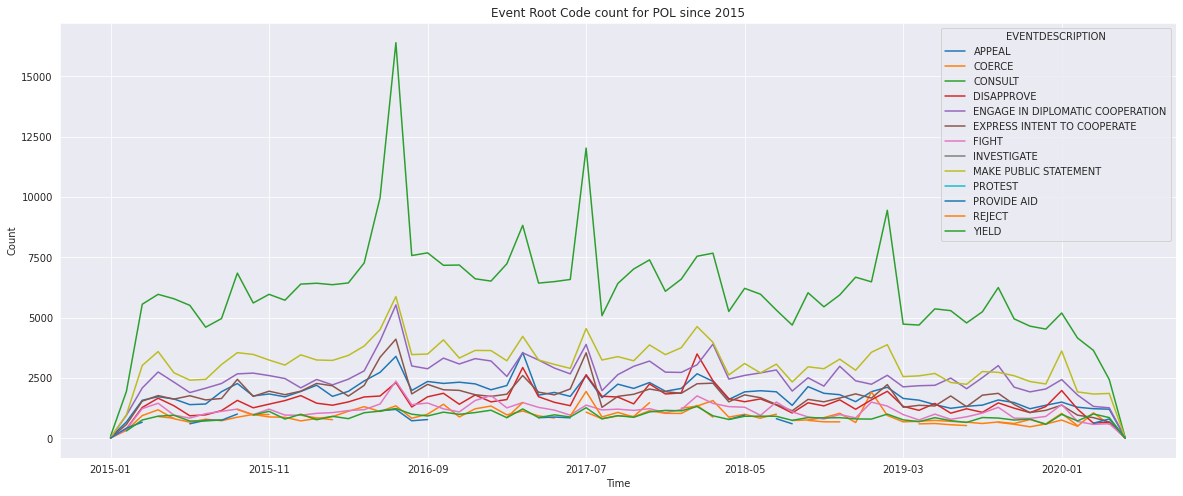
\includegraphics[width=\linewidth]{fig/PL/PLERCinTIME.png}
        \caption{Liczba zdarzeń z Polską dla poszczególnych kodów podstawowych w czasie - top 10. (źródło: opracowanie własne)}
        \label{fig:PLPERCinTIME}
    \end{figure}
    Na pierwszym miejscu w całym analizowanym okresie utrzymuje się kod \textit{CONSULT}.
    Następnymi w kolejności są kody \textit{MAKE PUBLIC STATEMENT} oraz \textit{ENGAGE IN DIPLOMATIC COOPERATION}.


    Wykres~\ref{fig:PLPERCpercinTIME} przedstawia procentową liczbę zdarzeń dla Polski dla poszczególnych kodów podstawowych w czasie.
    \begin{figure}[!htp]
        \centering
        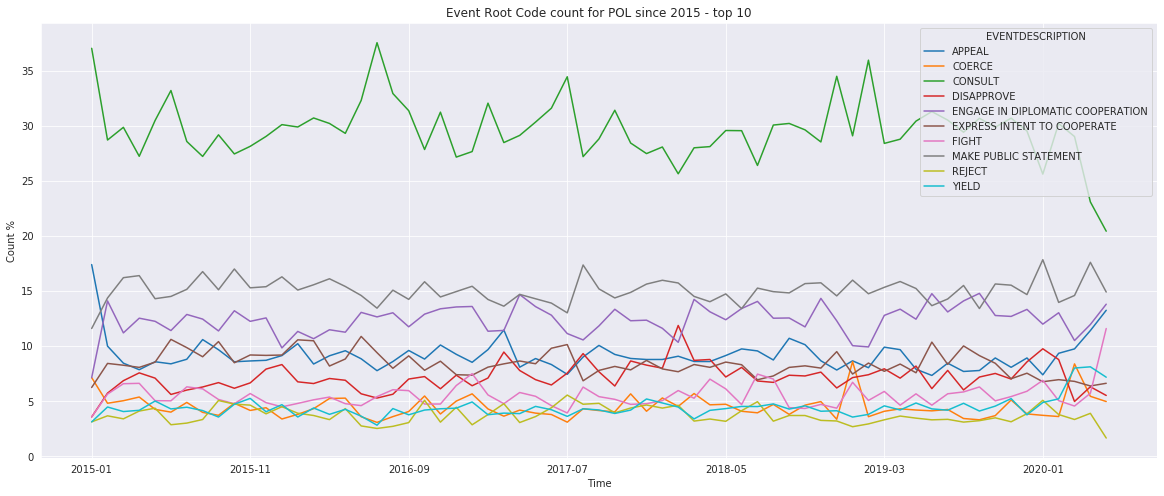
\includegraphics[width=\linewidth]{fig/PL/PLERCpercinTIME.png}
        \caption{Procentowa liczba zdarzeń z Polską dla poszczególnych kodów podstawowych w czasie - top 10. (źródło: opracowanie własne)}
        \label{fig:PLPERCpercinTIME}
    \end{figure}
    Proporcja poszczególnych kodów podstawowych utrzymuje się w analizowanym okresie na podobnym poziomie.

    \paragraph{Podstawowe kody zdarzeń między Polską a wybranymi krajami}

    Wykres~\ref{fig:PLDEUERC} przedstawia liczbę zdarzeń z Polską i~Niemcami dla poszczególnych kodów podstawowych w czasie.
    \begin{figure}[!htp]
        \centering
        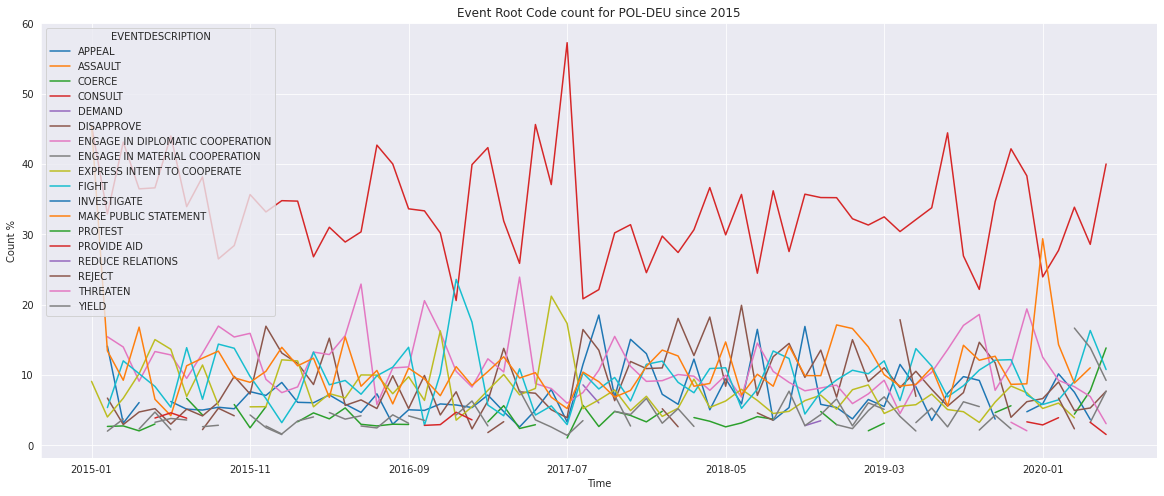
\includegraphics[width=\linewidth]{fig/PL/POLDEUERCperc.png}
        \caption{Procentowa liczba zdarzeń z Polska i~Niemcami dla poszczególnych kodów podstawowych w czasie - top 10. (źródło: opracowanie własne)}
        \label{fig:PLDEUERC}
    \end{figure}
    W analizowanym okresie dominuje kod podstawowy \textit{CONSULT}, który tylko w styczniu 2020 roku jest wyprzedzany przez od \textit{MAKE PUBLIC STATEMENT}.
    Pozostałe kody utrzymują się na niższym poziomie i~podlegają dynamicznym zmianom.

    Wykres~\ref{fig:PLFRAERC} przedstawia liczbę zdarzeń z Polską i~Francją dla poszczególnych kodów podstawowych w czasie.
    \begin{figure}[!htp]
        \centering
        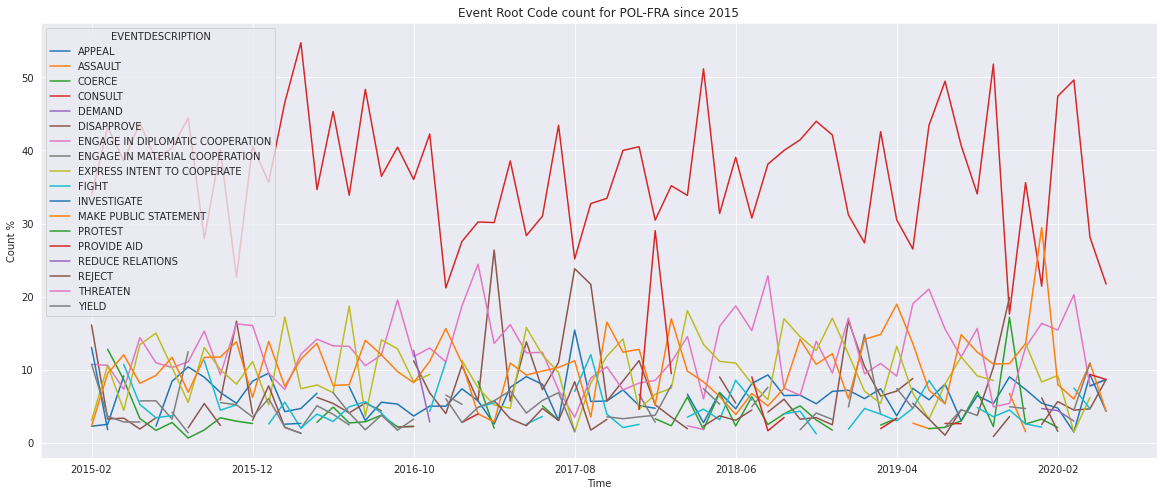
\includegraphics[width=\linewidth]{fig/PL/POLFRAERCperc.png}
        \caption{Procentowa liczba zdarzeń z Polską i~Francją dla poszczególnych kodów podstawowych w czasie - top 10. (źródło: opracowanie własne)}
        \label{fig:PLFRAERC}
    \end{figure}
    Tak jak w przypadku wykresu~\ref{fig:PLDEUERC} dla Polski i~Niemiec, na pierwszym miejscu utrzymuje się kod podstawowy \textit{CONSULT}.
    Pozostałe kody są mniej popularne i~podlegają ciągłym zmianom.

    Wykres~\ref{fig:PLGBRERC} przedstawia liczbę zdarzeń z Polską i~Wielką Brytanią dla poszczególnych kodów podstawowych w czasie.
    \begin{figure}[!htp]
        \centering
        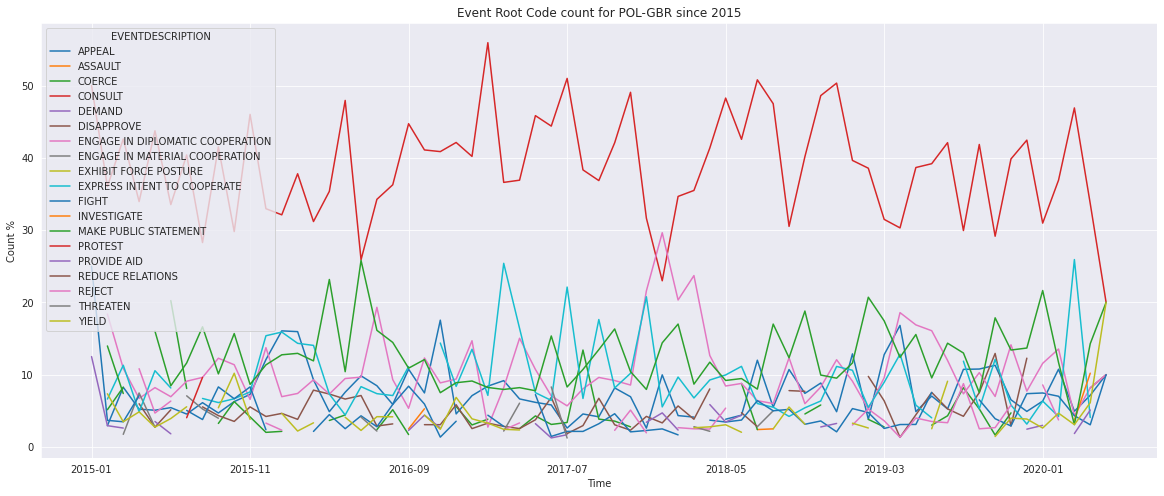
\includegraphics[width=\linewidth]{fig/PL/POLGBRERCperc.png}
        \caption{Procentowa liczba zdarzeń z Polską i~Wielka Brytanią dla poszczególnych kodów podstawowych w czasie - top 10. (źródło: opracowanie własne)}
        \label{fig:PLGBRERC}
    \end{figure}
    Podobnie jak na poprzednich wykresach, dominują zdarzenia \textit{CONSULT}.

    Wykres~\ref{fig:PLRUSERC} przedstawia liczbę zdarzeń z Polską i~Rosją dla poszczególnych kodów podstawowych w czasie.
    \begin{figure}[!htp]
        \centering
        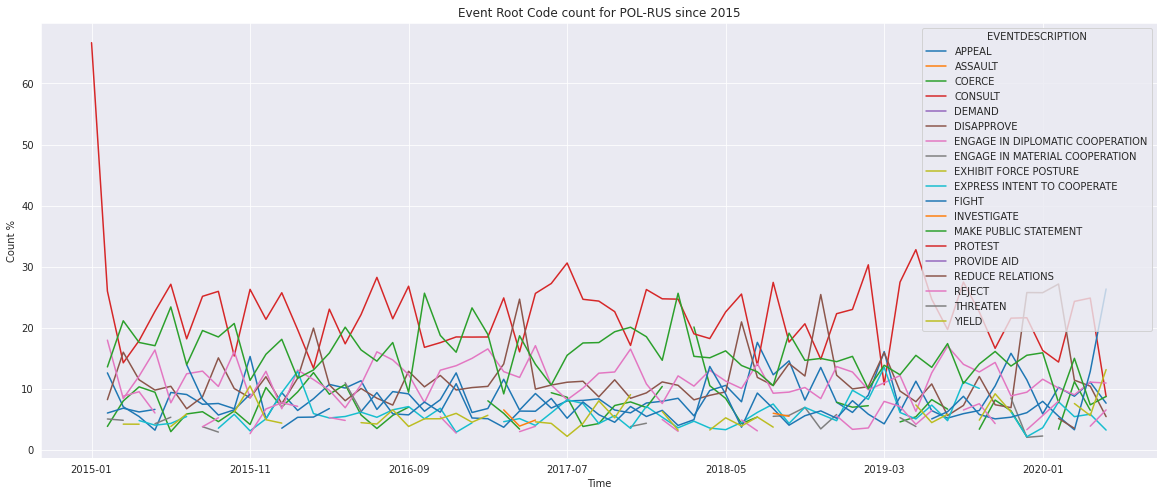
\includegraphics[width=\linewidth]{fig/PL/POLRUSERCperc.png}
        \caption{Procentowa liczba zdarzeń z Polską i~Rosją dla poszczególnych kodów podstawowych w czasie - top 10. (źródło: opracowanie własne)}
        \label{fig:PLRUSERC}
    \end{figure}
    Ponownie dominują zdarzenia \textit{CONSULT} jednak są zbliżone do pozostałych.
    Zauważalne jest częstsze występowanie kodów \textit{MAKE PUBLIC STATEMENT} oraz \textit{DISAPPROVE}.

    \subsection{Niemcy}

    \paragraph{Kraj para do zdarzenia}

    Wykres~\ref{fig:DEUpair} przedstawia liczbę zdarzeń dla Niemiec w których parą jest dany kraj.
    \begin{figure}[!htp]
        \centering
        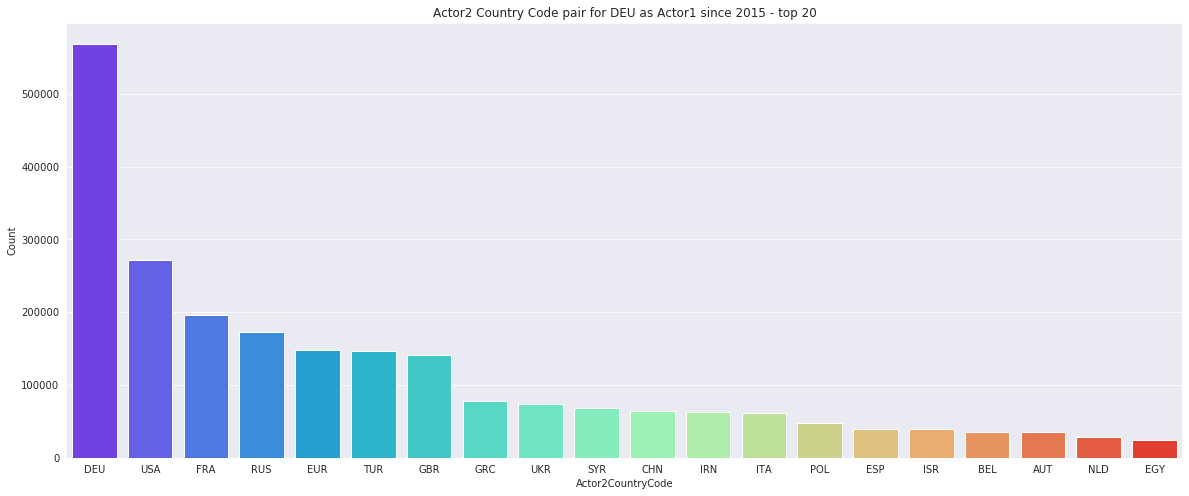
\includegraphics[width=\linewidth]{fig/DEU/DEUactor2Pair.png}
        \caption{Liczba zdarzeń z Niemcami w których parą jest dany kraj - top 20. (źródło: opracowanie własne)}
        \label{fig:DEUpair}
    \end{figure}
    Obserwujemy prawie dwukrotnie większą ilość zdarzeń w których parą dla Niemiec są one same, od następnych w kolejności Stanów Zjednoczonych.
    Często występującą parą w zdarzeniach są też Francja i~Rosja.

    Wykres~\ref{fig:DEUpairPerc} przedstawia procentową liczbę zdarzeń dla Niemiec w których parą jest dany kraj w czasie.
    \begin{figure}[!htp]
        \centering
        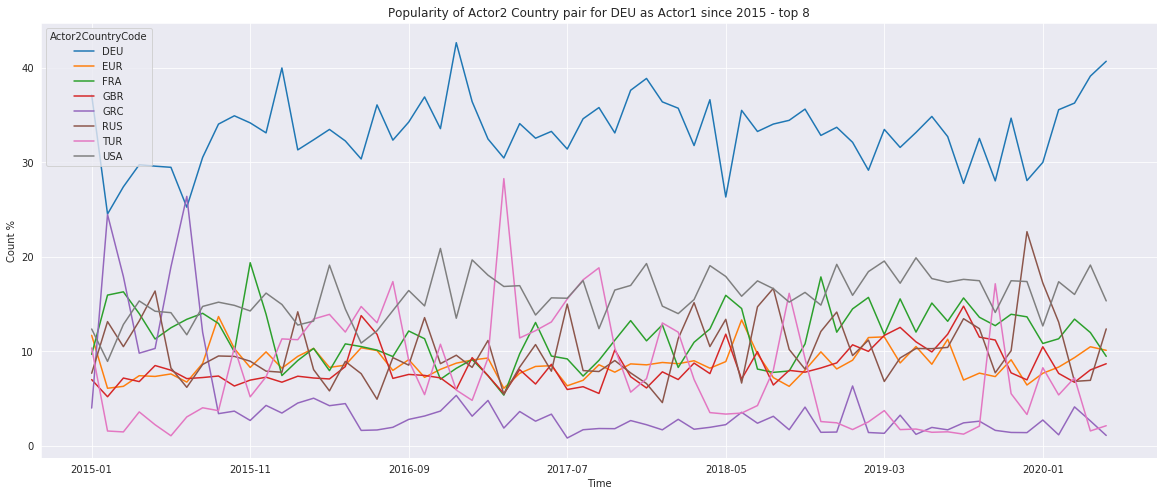
\includegraphics[width=\linewidth]{fig/DEU/DEUactor2PairPercinTIME.png}
        \caption{Procentowa liczba zdarzeń w których parą jest dany kraj w czasie. (źródło: opracowanie własne)}
        \label{fig:DEUpairPerc}
    \end{figure}
    Obserwujemy okresowe zwiększenie ilości zdarzeń Niemiec w parze z Grecją, Turcją oraz Rosją.
    Wyraźnym trendem jest duża ilość zdarzeń w parze ze Stanami Zjednoczonymi Ameryki.

    \paragraph{Podstawowy kod zdarzeń}

    Wykres~\ref{fig:DEUPERC} przedstawia liczbę zdarzeń z Niemcami dla poszczególnych kodów podstawowych od 2015 roku.
    \begin{figure}[!htp]
        \centering
        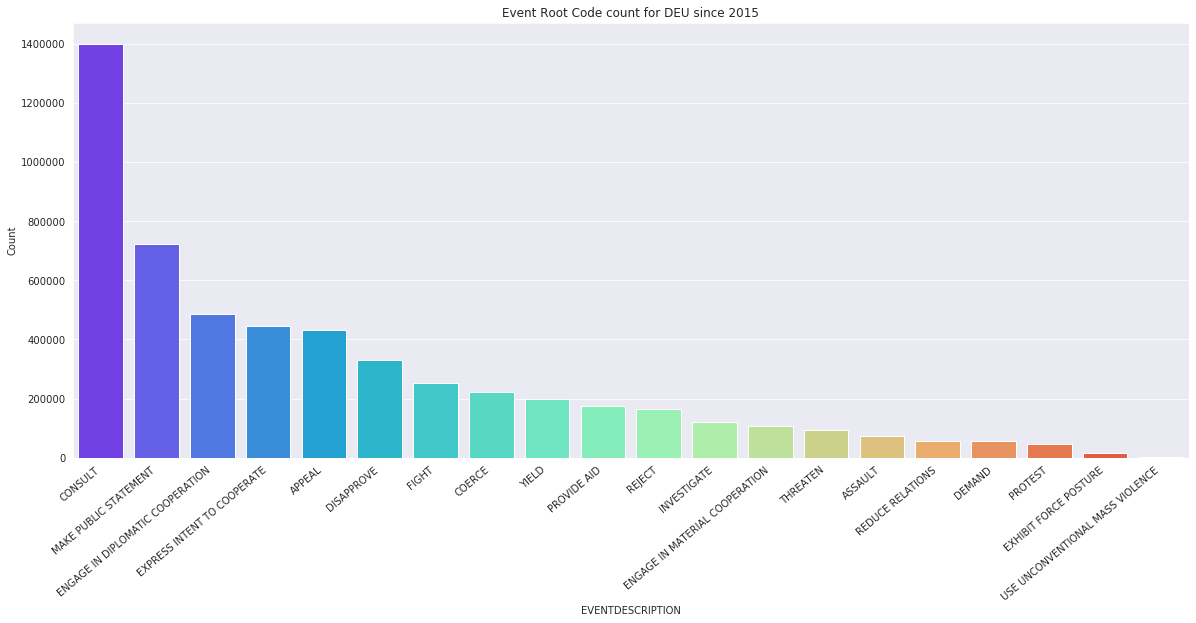
\includegraphics[width=\linewidth]{fig/DEU/DEUERC.png}
        \caption{Liczba zdarzeń z Niemcami dla poszczególnych kodów podstawowych od 2015 roku. (źródło: opracowanie własne)}
        \label{fig:DEUPERC}
    \end{figure}
    Obserwujemy dwukrotnie większą ilość zdarzeń \textit{CONSULT} niż następnymi w kolejności zdarzeniami \textit{MAKE PUBLIC STATEMENT}.
    Często występują też zdarzenia \textit{ENGAGE IN DIPLOMATIC COOPERATION} oraz \textit{EXPRESS INTENT TO COOPERATE}.


    Wykres~\ref{fig:DEUPERCinTIME} przedstawia liczbę zdarzeń z Niemcami dla poszczególnych kodów podstawowych w czasie - top 10.
    \begin{figure}[!htp]
        \centering
        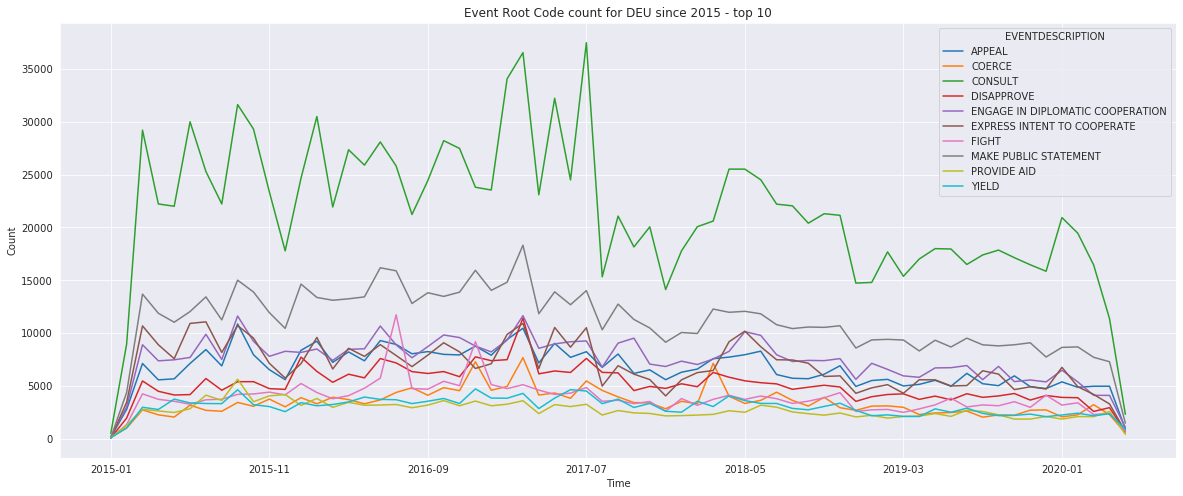
\includegraphics[width=\linewidth]{fig/DEU/DEUERCinTIME.png}
        \caption{Liczba zdarzeń z Niemcami dla poszczególnych kodów podstawowych w czasie - top 10. (źródło: opracowanie własne)}
        \label{fig:DEUPERCinTIME}
    \end{figure}
    W całym analizowanym okresie dominują kody podstawowe \textit{CONSULT} oraz \textit{MAKE PUBLIC STATEMENT}.

    Wykres~\ref{fig:DEUPERCpercinTIME} przedstawia procentową liczbę zdarzeń z Niemcami dla poszczególnych kodów podstawowych w czasie.
    \begin{figure}[!htp]
        \centering
        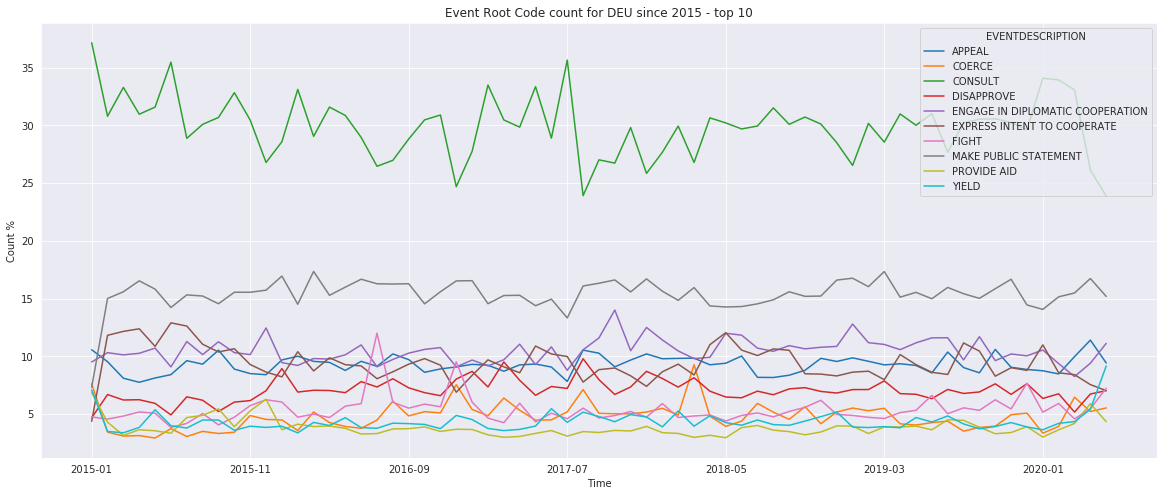
\includegraphics[width=\linewidth]{fig/DEU/DEUERCpercinTIME.png}
        \caption{Procentowa liczba zdarzeń z Niemcami dla poszczególnych kodów podstawowych w czasie - top 10. (źródło: opracowanie własne)}
        \label{fig:DEUPERCpercinTIME}
    \end{figure}
    Proporcja poszczególnych kodów podstawowych w analizowanym okresie utrzymuje się.
    Wyraźnie dominuje kod podstawowy \textit{CONSULT}.

    \paragraph{Podstawowe kody zdarzeń między Niemcami a wybranymi krajami}

    Wykres~\ref{fig:DEUPOLERC} przedstawia liczbę zdarzeń z Niemcami i~Polską dla poszczególnych kodów podstawowych w czasie.
    \begin{figure}[!htp]
        \centering
        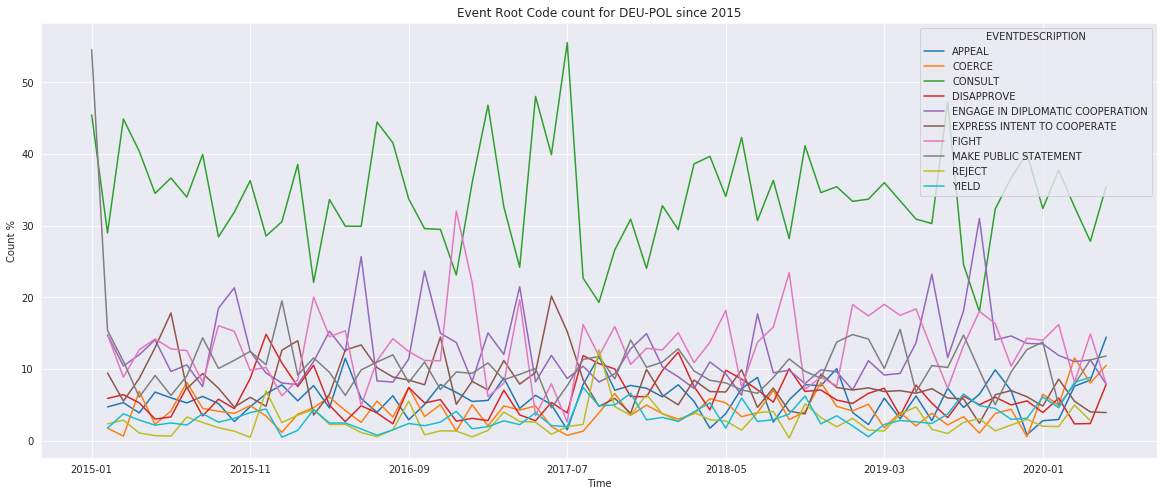
\includegraphics[width=\linewidth]{fig/DEU/DEUPOLERCperc.png}
        \caption{Procentowa liczba zdarzeń z Niemcami i~Polską dla poszczególnych kodów podstawowych w czasie. (źródło: opracowanie własne)}
        \label{fig:DEUPOLERC}
    \end{figure}
    W całym analizowanym okresie dominują zdarzenia podstawowe \textit{CONSULT}.
    Obserwujemy też duża ilość zdarzeń podstawowych \textit{FIGHT}.
    Może być to spowodowane dużą ilością zdarzeń mających na celu upamiętnienie historycznych działań wojennych.

    Wykres~\ref{fig:DEURUSERC} przedstawia liczbę zdarzeń z Niemcami i~Rosją dla poszczególnych kodów podstawowych w czasie.
    \begin{figure}[!htp]
        \centering
        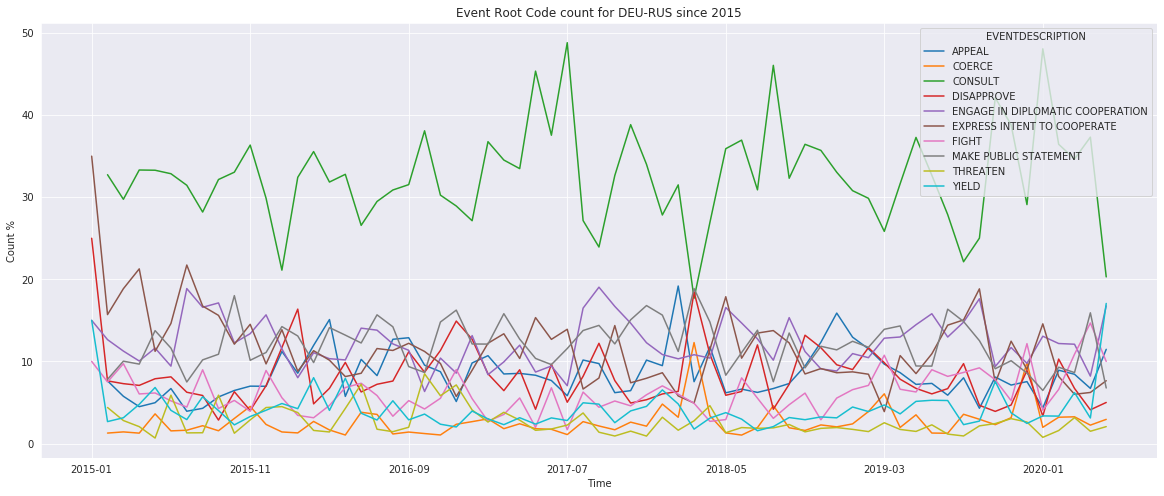
\includegraphics[width=\linewidth]{fig/DEU/DEURUSERCperc.png}
        \caption{Procentowa liczba zdarzeń z Niemcami i~Rosją dla poszczególnych kodów podstawowych w czasie. (źródło: opracowanie własne)}
        \label{fig:DEURUSERC}
    \end{figure}
    Dominującym jest kod podstawowy \textit{CONSULT}.
    Obserwujemy okresy wyraźnego zwiększenia ilości zdarzeń z kodem podstawowym \textit{DISAPPROVE} i~w tym samym czasie zmniejszenia zdarzeń \textit{CONSULT}.

    \subsection{Rosja}

    \paragraph{Kraj para do zdarzenia}

    Wykres~\ref{fig:RUSpair} przedstawia liczbę zdarzeń dla Rosji w których parą jest dany kraj od 2015 roku.

    \begin{figure}[!htp]
        \centering
        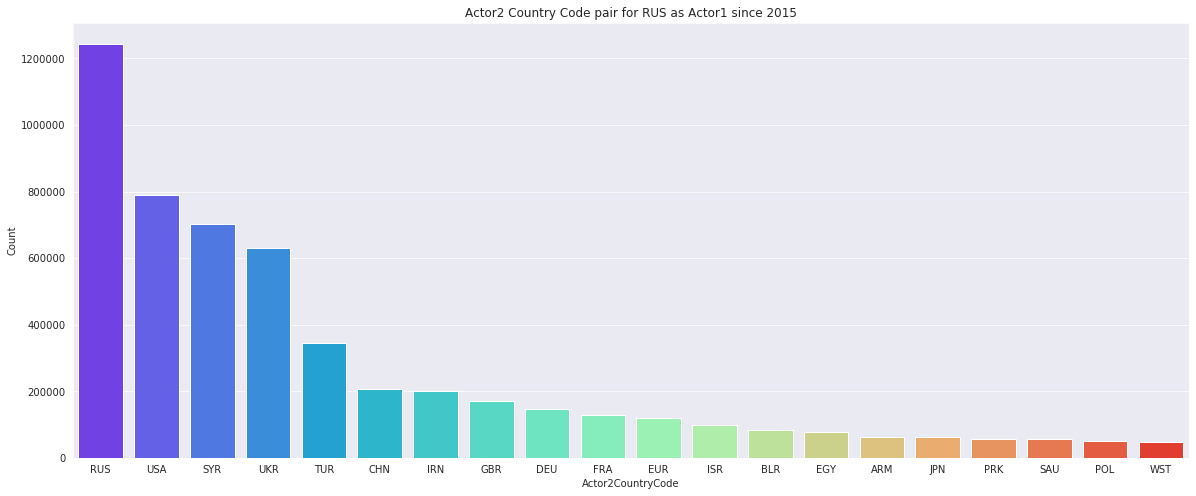
\includegraphics[width=\linewidth]{fig/RUS/RUSactor2Pair.png}
        \caption{Liczba zdarzeń z Rosją w których parą jest dany kraj od 2015 roku. (źródło: opracowanie własne)}
        \label{fig:RUSpair}
    \end{figure}
    W porównaniu z wcześniej analizowanymi państwami gdzie drugi w kolejności kraj miał o~połowę mniej zdarzeń, w przypadku Rosji zdarzeń jest tylko o~1/3 mniej.
    Najpopularniejszymi parami do zdarzeń dla Rosji, prócz niej samej, są Stany Zjednoczone Ameryki, Syria oraz Ukraina.

    Wykres~\ref{fig:RUSpairPerc} przedstawia procentową liczbę zdarzeń dla Rosji w których parą jest dany kraj w czasie.
    \begin{figure}[!htp]
        \centering
        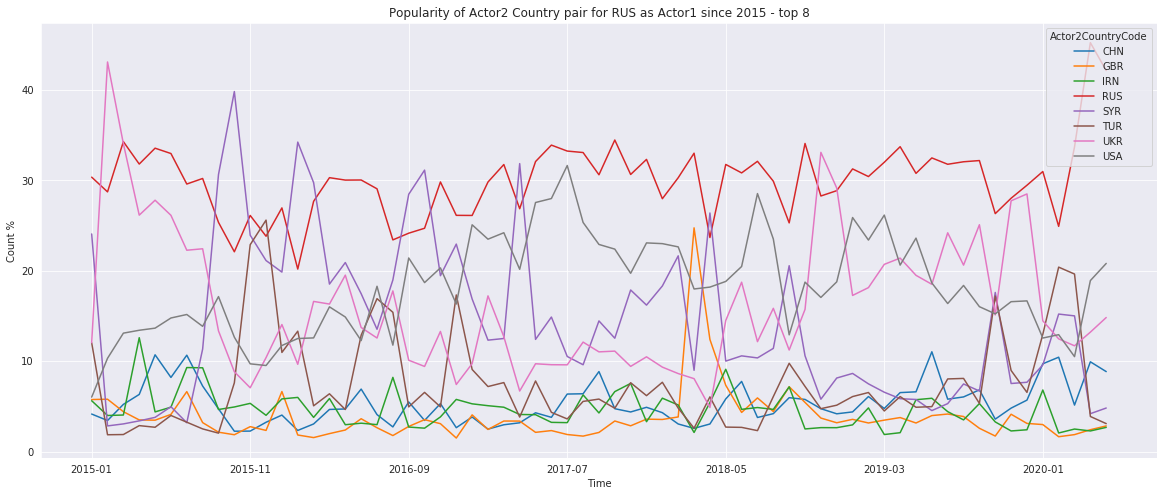
\includegraphics[width=\linewidth]{fig/RUS/RUSactor2PairPercinTIME.png}
        \caption{Procentowa liczba zdarzeń dla Rosji w których parą jest dany kraj w czasie - top 8. (źródło: opracowanie własne)}
        \label{fig:RUSpairPerc}
    \end{figure}
    Obserwujemy okresową dominację zdarzeń w których parą jest Ukraina, Syria oraz Turcja.

    \paragraph{Podstawowy kod zdarzeń}

    Wykres~\ref{fig:RUSPERC} przedstawia liczbę zdarzeń dla Rosji dla poszczególnych kodów podstawowych pd 2015 roku.

    \begin{figure}[!htp]
        \centering
        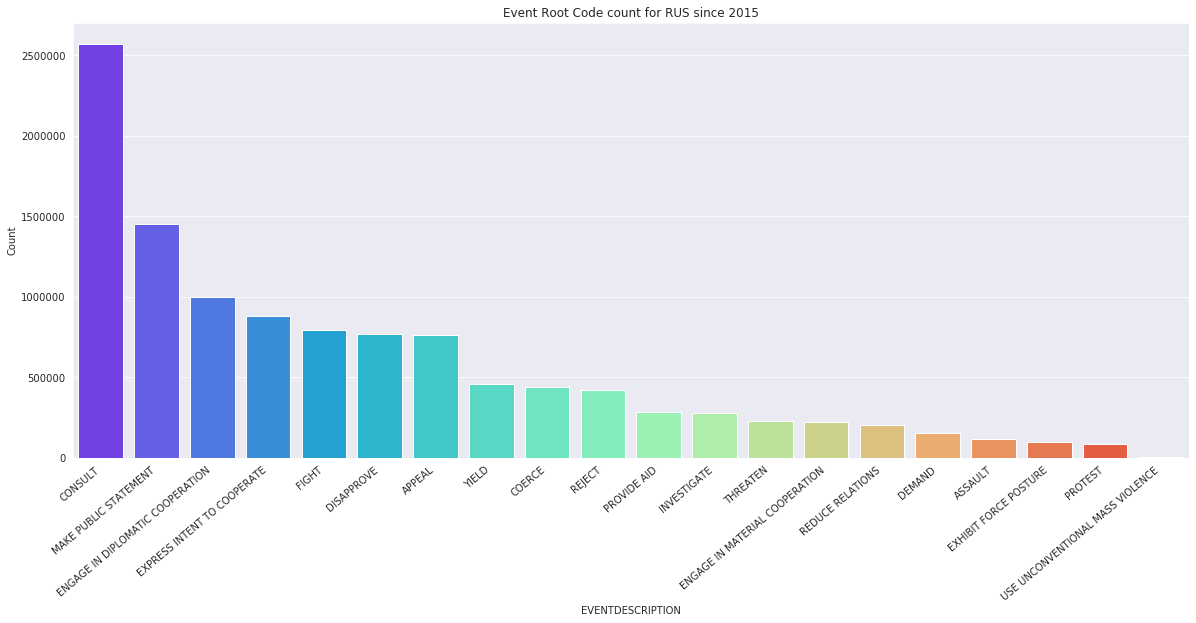
\includegraphics[width=\linewidth]{fig/RUS/RUSERC.png}
        \caption{Liczba zdarzeń dla poszczególnych kodów podstawowych od 2015 roku. (źródło: opracowanie własne)}
        \label{fig:RUSPERC}
    \end{figure}
    Najliczniej występują zdarzenia z kodami podstawowymi \textit{CONSULT, MAKE PUBLIC STATEMENT} oraz \textit{ENGAGE IN DIPLOMATIC COOPERATION}.

    Wykres~\ref{fig:RUSPERCinTIME} przedstawia liczbę zdarzeń z Rosją dla poszczególnych kodów podstawowych w czasie.
    \begin{figure}[!htp]
        \centering
        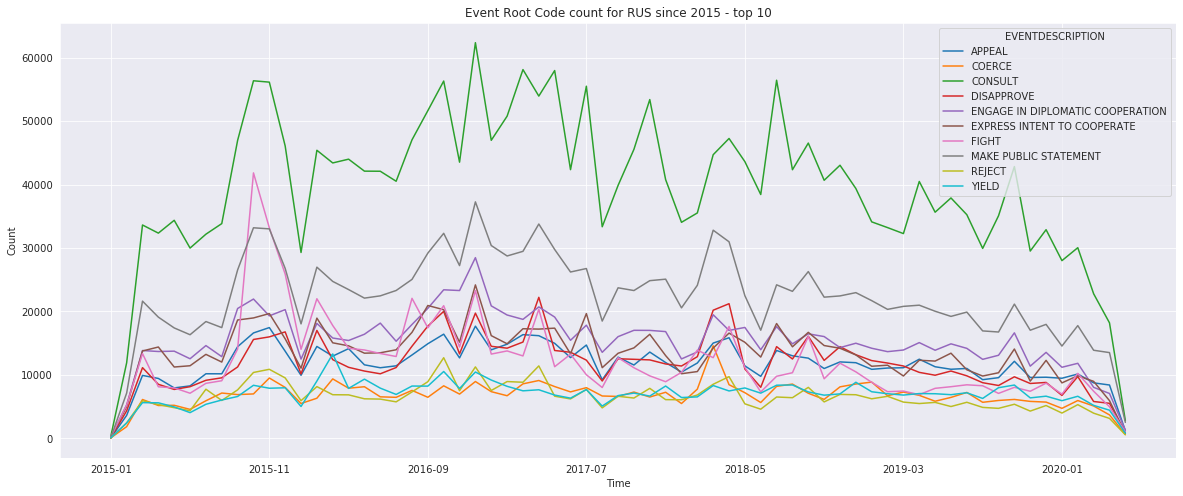
\includegraphics[width=\linewidth]{fig/RUS/RUSERCinTIME.png}
        \caption{Liczba zdarzeń dla poszczególnych kodów podstawowych w czasie - top 10. (źródło: opracowanie własne)}
        \label{fig:RUSPERCinTIME}
    \end{figure}
    Dominuje występowanie kodu podstawowego \textit{CONSULT}.
    Na drugim miejscu znajduje się kod \textit{EXPRESS INTENT TO COOPERATE}, tylko przez moment wyprzedzony przez kod \textit{FIGHT}.


    Wykres~\ref{fig:RUSPERCpercinTIME} przedstawia procentową liczbę zdarzeń z Rosją dla poszczególnych kodów podstawowych w czasie.
    \begin{figure}[!htp]
        \centering
        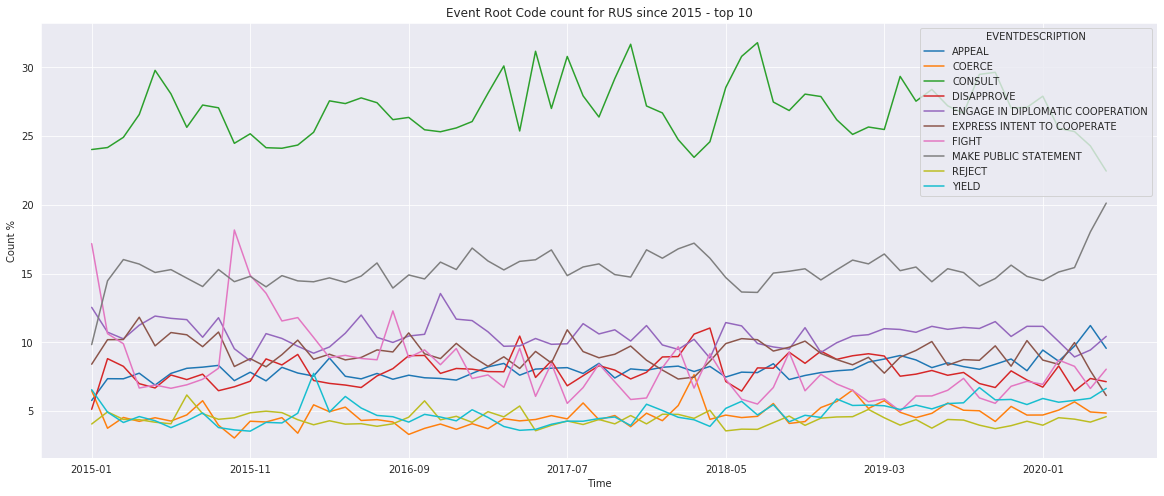
\includegraphics[width=\linewidth]{fig/RUS/RUSERCpercinTIME.png}
        \caption{Procentowa liczba zdarzeń z Rosją dla poszczególnych kodów podstawowych w czasie - top 10. (źródło: opracowanie własne)}
        \label{fig:RUSPERCpercinTIME}
    \end{figure}
    Stosunek występowania poszczególnych kodów pozostaje na podobnym poziomie.
    Wyraźnym odstępstwem jest czasowe zwiększenie popularności kodu podstawowego \textit{FIGHT}.

    \paragraph{Podstawowe kody zdarzeń między Rosją a wybranymi krajami}

    Wykres~\ref{fig:RUSPOLERC} przedstawia liczbę zdarzeń z Rosją i~Polską dla poszczególnych kodów podstawowych w czasie.
    \begin{figure}[!htp]
        \centering
        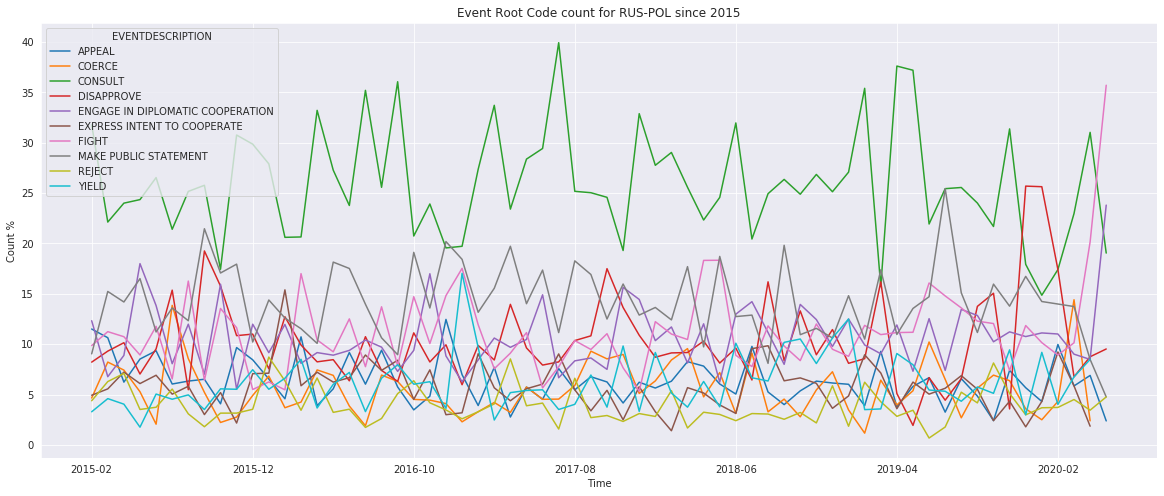
\includegraphics[width=\linewidth]{fig/RUS/RUSPOLERCperc.png}
        \caption{Procentowa liczba zdarzeń z Rosją i~Niemcami dla poszczególnych kodów podstawowych w czasie - top 10. (źródło: opracowanie własne)}
        \label{fig:RUSPOLERC}
    \end{figure}
    W wydarzeniach w których uczestniczy Rosja i~Polska obserwujemy dominację kodu podstawowego \textit{CONSULT}.
    Występują wyraźne okresy zwiększenia popularności kodów \textit{DISAPPROVE} oraz \textit{MAKE PUBLIC STATEMENT} przy jednoczesnym zmniejszeniu popularności kodu \textit{CONSULT}.

    Wykres~\ref{fig:RUSRUSERC} przedstawia liczbę zdarzeń z Rosją i~Niemcami dla poszczególnych kodów podstawowych w czasie.
    \begin{figure}[!htp]
        \centering
        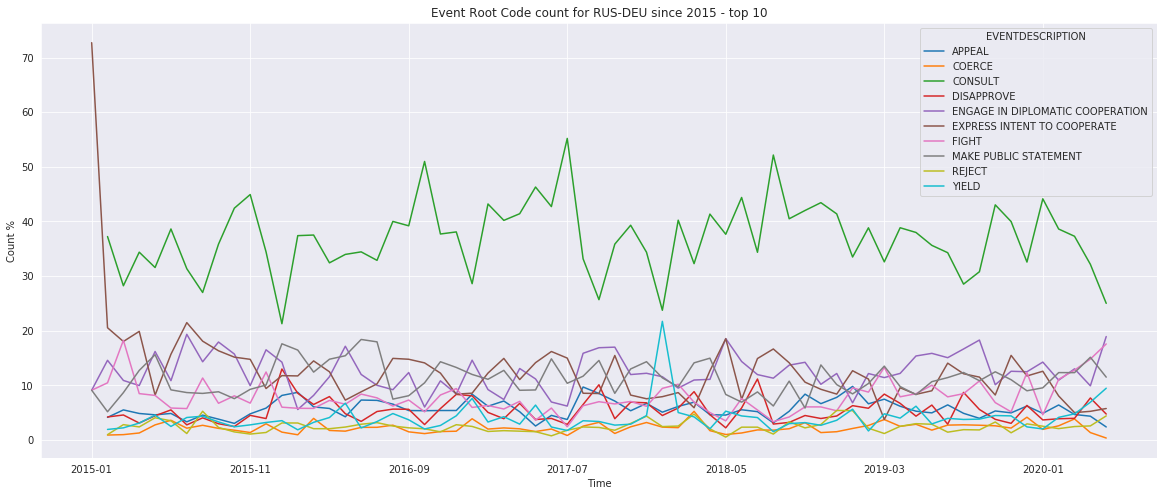
\includegraphics[width=\linewidth]{fig/RUS/RUSDEUERCperc.png}
        \caption{Procentowa liczba zdarzeń z Rosją i~Niemcami dla poszczególnych kodów podstawowych w czasie - top 10. (źródło: opracowanie własne)}
        \label{fig:RUSRUSERC}
    \end{figure}
    Popularność kodu podstawowego \textit{CONSULT} w analizowanym okresie oscyluje w okolicach 40\%, podczas gdy pozostałych kodów utrzymuje się w większości poniżej 20\%.

    \subsection{Stan Zjednoczone}

    \paragraph{Kraj para do zdarzenia}

    Wykres~\ref{fig:USApair} przedstawia liczbę zdarzeń dla Stanów Zjednoczonych w których parą jest dany kraj.

    \begin{figure}[!htp]
        \centering
        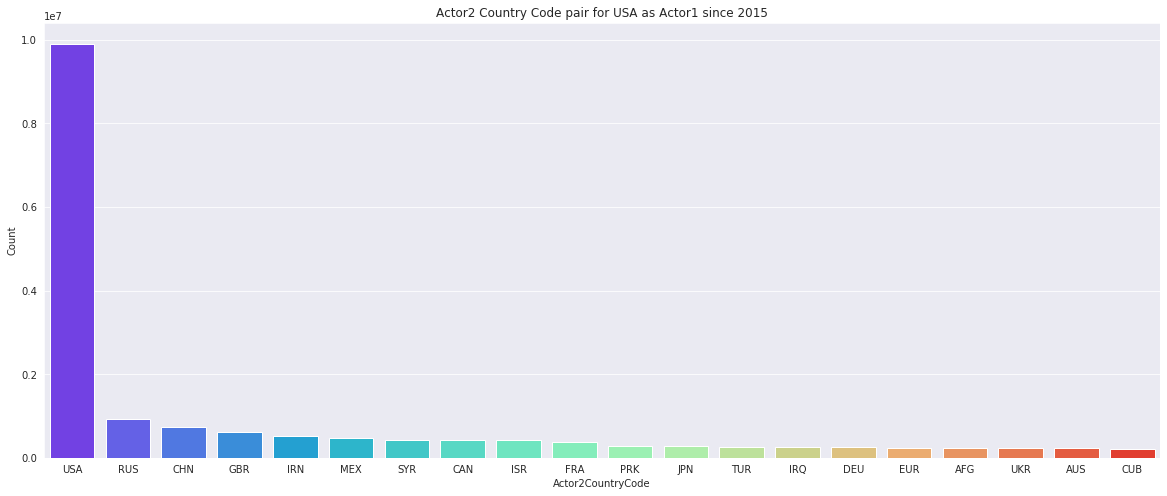
\includegraphics[width=\linewidth]{fig/USA/USAactor2Pair.png}
        \caption{Liczba zdarzeń ze Stanami Zjednoczonymi w których parą jest dany kraj od 2015 roku. (źródło: opracowanie własne)}
        \label{fig:USApair}
    \end{figure}
    Liczba zdarzeń w których parą dla Stanów Zjednoczonych są one same jest o~rząd wielkości większa od następnej w kolejności Rosji.
    Stany Zjednoczone mają też dużo zdarzeń w których parą są Chiny, Wielka Brytania, Iran oraz Meksyk.

    Wykres~\ref{fig:USApairPerc} przedstawia procentową liczbę zdarzeń dla Stanów Zjednoczonych w których parą jest dany kraj w czasie.
    \begin{figure}[!htp]
        \centering
        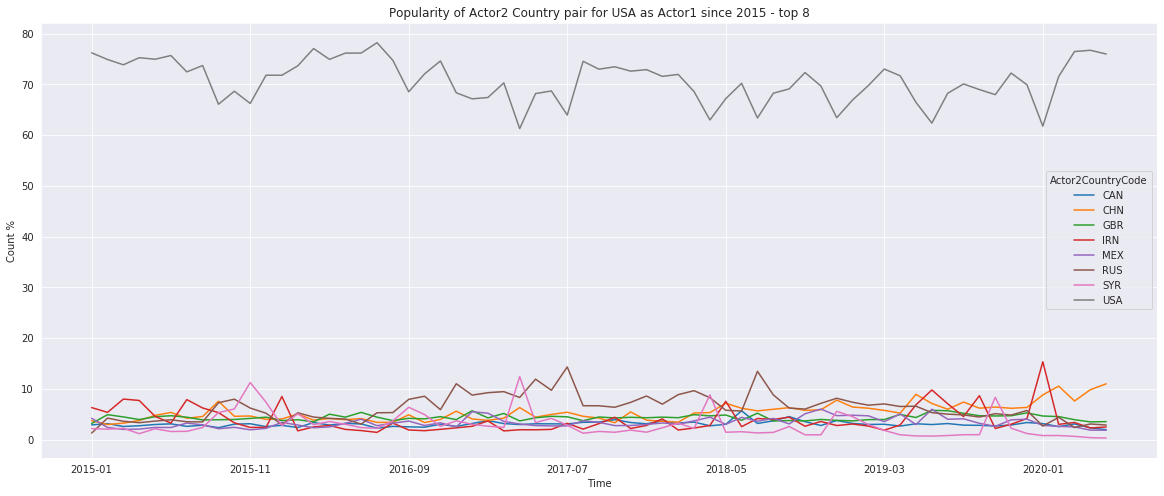
\includegraphics[width=\linewidth]{fig/USA/USAactor2PairPercinTIME.png}
        \caption{Procentowa liczba zdarzeń ze Stanami Zjednoczonymi w których parą jest dany kraj w czasie (z pominięciem USA)- top 10. (źródło: opracowanie własne)}
        \label{fig:USApairPerc}
    \end{figure}
    Przez większość analizowanego okresu główną parą do zdarzeń dla Stanów Zjednoczonych (z pominięciem ich samych) jest Rosja.
    Jako dominująca para do zdarzeń występują także Iran, Syria, Wielka Brytania, Chiny oraz Izrael.

    \paragraph{Podstawowy kod zdarzeń}

    Wykres~\ref{fig:USAPERC} przedstawia liczbę zdarzeń dla Stanów Zjednoczonych dla poszczególnych kodów podstawowych od 2015 roku.

    \begin{figure}[!htp]
        \centering
        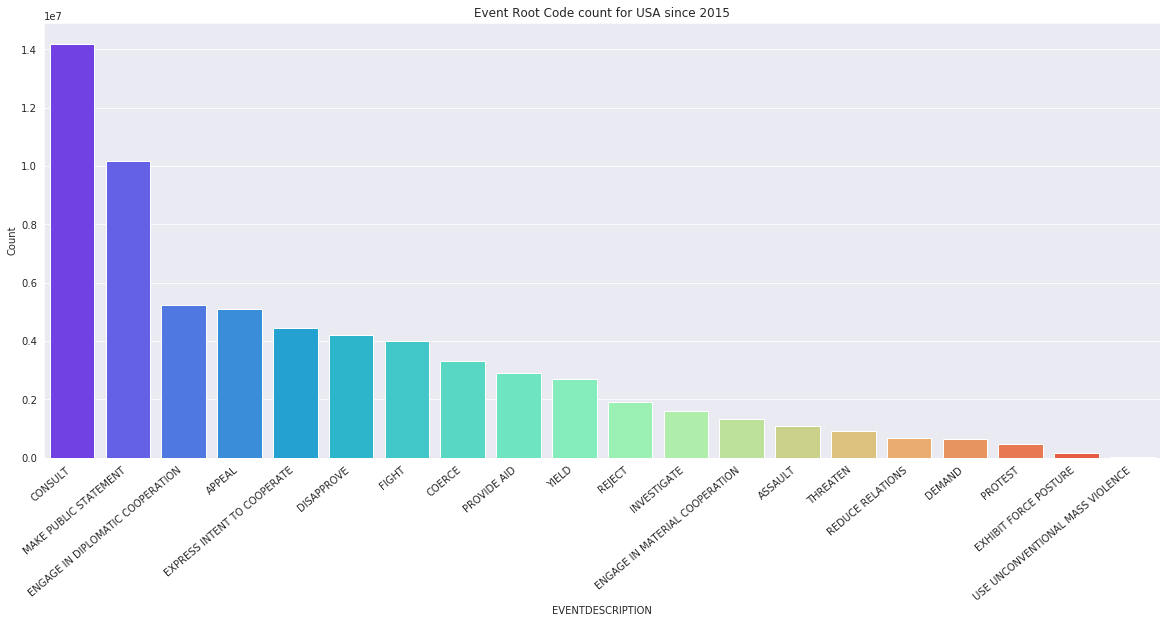
\includegraphics[width=\linewidth]{fig/USA/USAERC.png}
        \caption{Liczba zdarzeń ze Stanami Zjednoczonymi dla poszczególnych kodów podstawowych od 2015 roku. (źródło: opracowanie własne)}
        \label{fig:USAPERC}
    \end{figure}
    Tak jak w przypadku poprzednio analizowanych krajów dominują zdarzenia z kodem podstawowym \textit{CONSULT}.
    Kolejnymi kodami według liczby występujących zdarzeń są \textit{MAKE PUBLIC STATEMENT, ENGAGE IN DIPLOMATIC COOPERATION} oraz \textit{APPEAL}.

    Wykres~\ref{fig:USAPERCinTIME} przedstawia liczbę zdarzeń ze Stanami Zjednoczonymi dla poszczególnych kodów podstawowych w czasie.
    \begin{figure}[!htp]
        \centering
        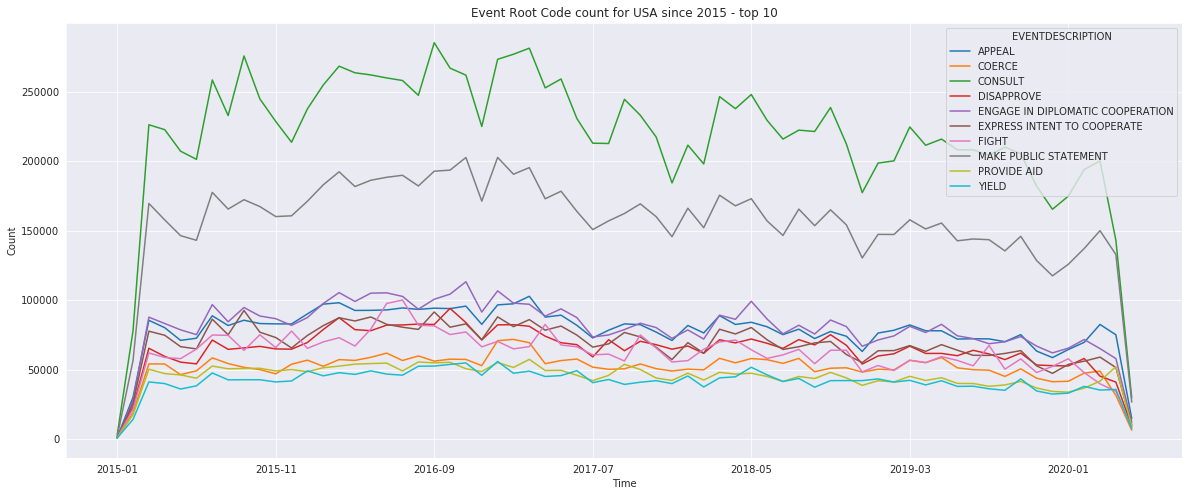
\includegraphics[width=\linewidth]{fig/USA/USAERCinTIME.png}
        \caption{Liczba zdarzeń ze Stanami Zjednoczonymi dla poszczególnych kodów podstawowych w czasie - top 10. (źródło: opracowanie własne)}
        \label{fig:USAPERCinTIME}
    \end{figure}
    W całym analizowanym okresie na pierwszych dwóch miejscach pod względem liczby zdarzeń występują kody \textit{CONSULT} oraz \textit{MAKE PUBLIC STATEMENT}.
    Pozostałe kody zdarzeń charakteryzują się znacznie mniejszą licznością zdarzeń.

    Wykres~\ref{fig:USAPERCpercinTIME} przedstawia procentową liczbę zdarzeń dla Stanów Zjednoczonych dla poszczególnych kodów podstawowych w czasie.
    \begin{figure}[!htp]
        \centering
        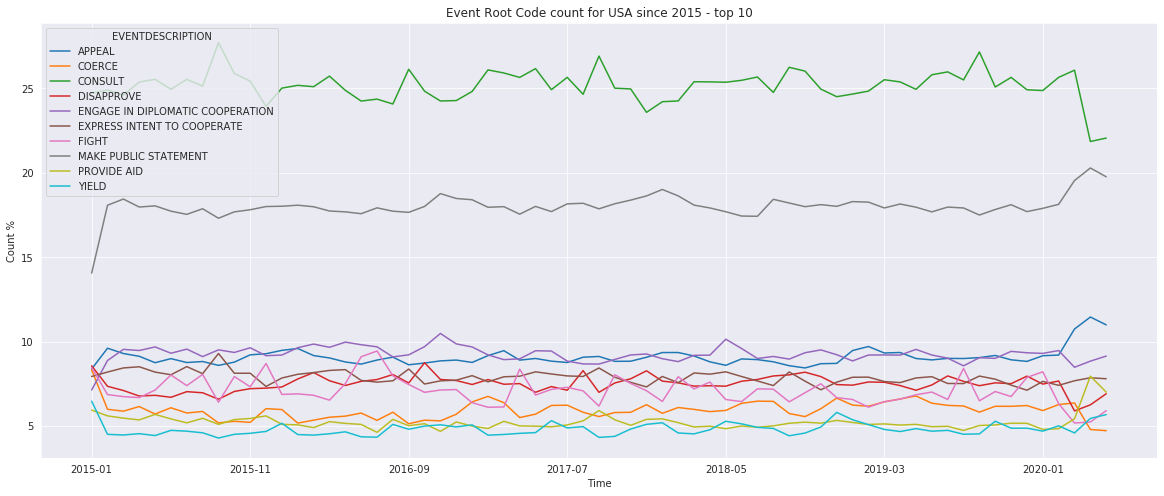
\includegraphics[width=\linewidth]{fig/USA/USAERCpercinTIME.png}
        \caption{Procentowa liczba zdarzeń ze Stanami Zjednoczonymi dla poszczególnych kodów podstawowych w czasie - top 10. (źródło: opracowanie własne)}
        \label{fig:USAPERCpercinTIME}
    \end{figure}
    Proporcja między kodami zdarzeń podstawowych w analizowanym okresie czasu pozostaje na podobnym poziomie.
    Dominują kod podstawowy \textit{CONSULT} (oscyluje w okolicach 25\%) oraz kod podstawowy \textit{MAKE PUBLIC STATEMENT} (oscyluje w okolicach 17\%).

    \paragraph{Podstawowe kody zdarzeń między Stanami Zjednoczonymi a wybranymi krajami}

    Wykres~\ref{fig:USAPOLERC} przedstawia liczbę zdarzeń ze Stanami Zjednoczonymi i~Polską dla poszczególnych kodów podstawowych w czasie.
    \begin{figure}[!htp]
        \centering
        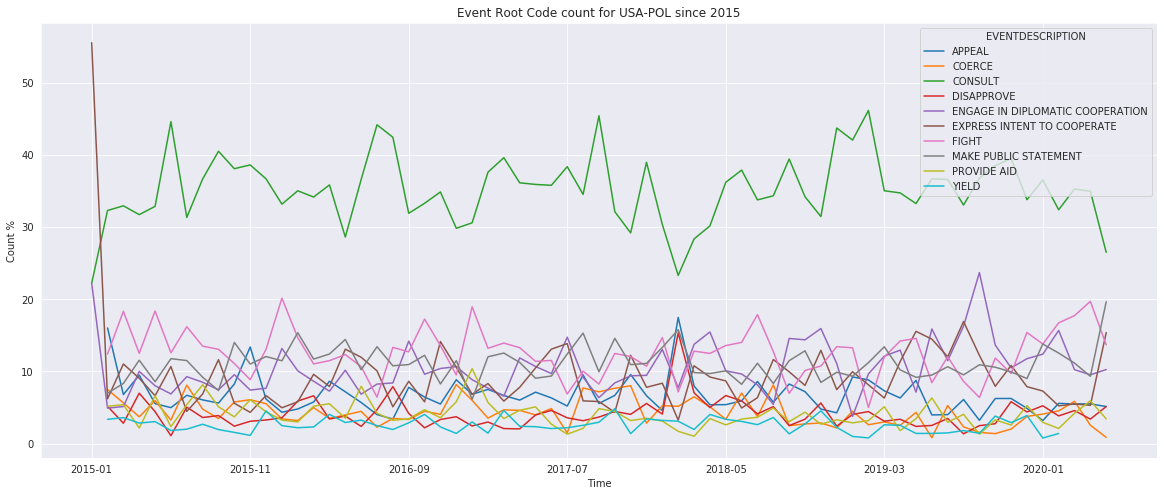
\includegraphics[width=\linewidth]{fig/USA/USAPOLERCperc.png}
        \caption{Procentowa liczba zdarzeń ze Stanami Zjednoczonymi i~Polską dla poszczególnych kodów podstawowych w czasie - top 10. (źródło: opracowanie własne)}
        \label{fig:USAPOLERC}
    \end{figure}
    Obserwujemy dominację zdarzeń z kodem podstawowym \textit{CONSULT} z popularnością oscylującą około 40\%.
    Pozostałe kody w analizowanym okresie utrzymują się głównie poniżej 20\% wystąpień.

    Wykres~\ref{fig:USADEUERC} przedstawia liczbę zdarzeń ze Stanami Zjednoczonymi i~Niemcami dla poszczególnych kodów podstawowych w czasie.
    \begin{figure}[!htp]
        \centering
        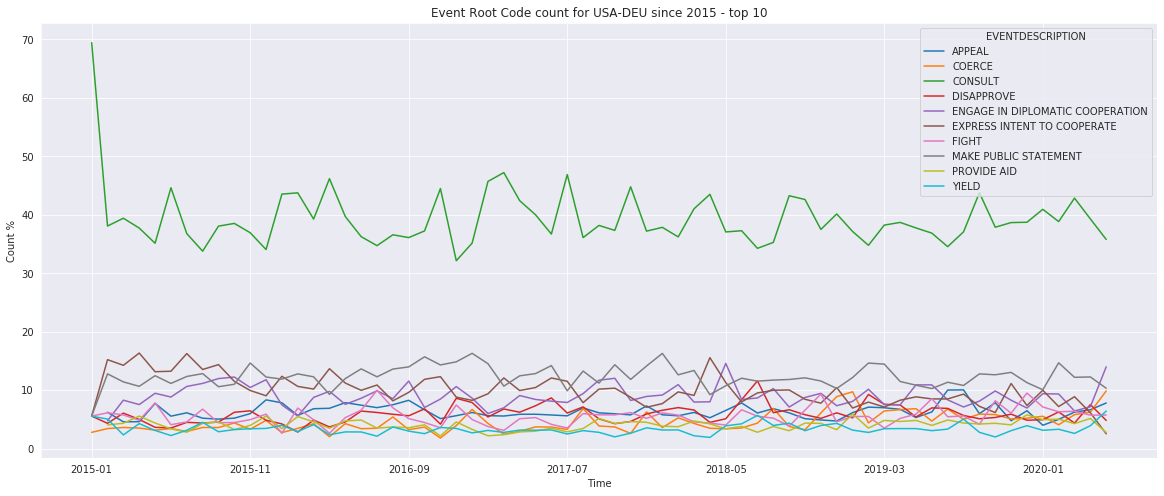
\includegraphics[width=\linewidth]{fig/USA/USADEUERCperc.png}
        \caption{Procentowa liczba zdarzeń ze Stanami Zjednoczonymi i~Niemcami dla poszczególnych kodów podstawowych w czasie - top 10. (źródło: opracowanie własne)}
        \label{fig:USADEUERC}
    \end{figure}
    W porównaniu z poprzednim wykresem~\ref{fig:USAPOLERC} obserwujemy jeszcze większą dominację zdarzeń z kodem podstawowym \textit{CONSULT}.
    Pozostałe kody w analizowanym okresie utrzymują się głównie poniżej 15\% wystąpień.

    Wykres~\ref{fig:USARUSERC} przedstawia liczbę zdarzeń ze Stanami Zjednoczonymi i~Rosją dla poszczególnych kodów podstawowych w czasie.
    \begin{figure}[!htp]
        \centering
        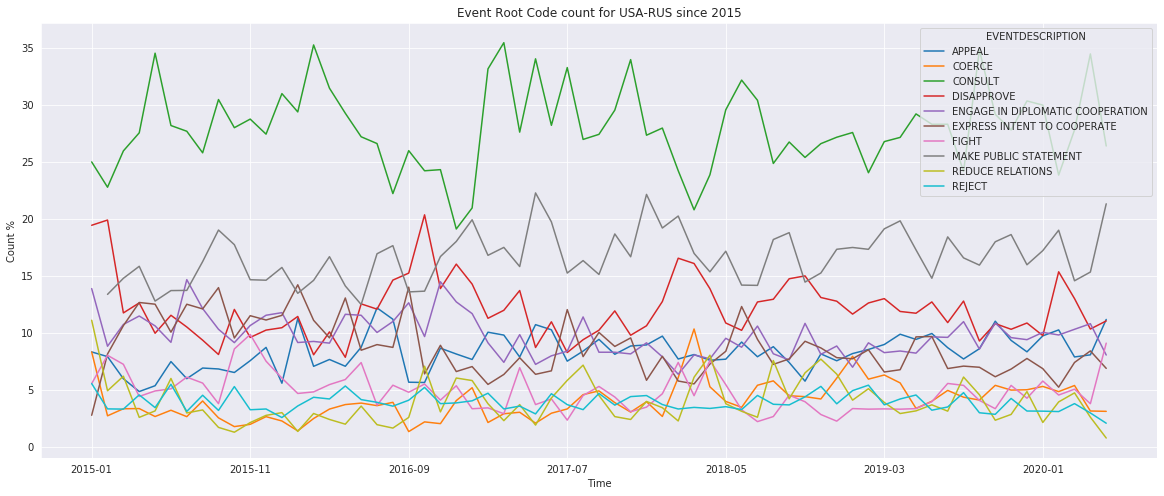
\includegraphics[width=\linewidth]{fig/USA/USARUSERCperc.png}
        \caption{Procentowa liczba zdarzeń ze Stanami Zjednoczonymi i~Rosją dla poszczególnych kodów podstawowych w czasie - top 10. (źródło: opracowanie własne)}
        \label{fig:USARUSERC}
    \end{figure}
    Obserwujemy mniejszy niż na poprzednich wykresach~\ref{fig:USAPOLERC},~\ref{fig:USADEUERC} odstęp pomiędzy popularnością zdarzeń z kodem \textit{CONSULT} a następnymi w kolejności \textit{MAKE PUBLIC STATEMENT} oraz \textit{DISAPPROVE}.


    \section{Analiza siły powiązania}\label{sec:analiza-siły-powiązania}
    W tej części przeanalizowana zostanie siła powiązania pomiędzy wybranymi krajami, a także jej symetryczność.
    Siła powiązania, zaproponowana w artykule~\cite{Yuan2017}, obliczana jest jako stosunek liczby zdarzeń pomiędzy krajem A, a krajem B, do liczby wszystkich zdarzeń w których kraj A jest aktorem 1.
    Ponieważ siła powiązania nie jest znormalizowana przez liczbę zdarzeń dla kraju B, dlatego nie jest symetryczna.
    Odzwierciedla to jak ważny dla kraju A jest kraj B.

    \subsection{Analiza siły powiązania miedzy wybranymi krajami}

    \paragraph{Polska}

    Wykres~\ref{fig:PLConnection} przedstawia siłę połączenia Polski z wybranymi krajami w czasie.
    \begin{figure}[!htp]
        \centering
        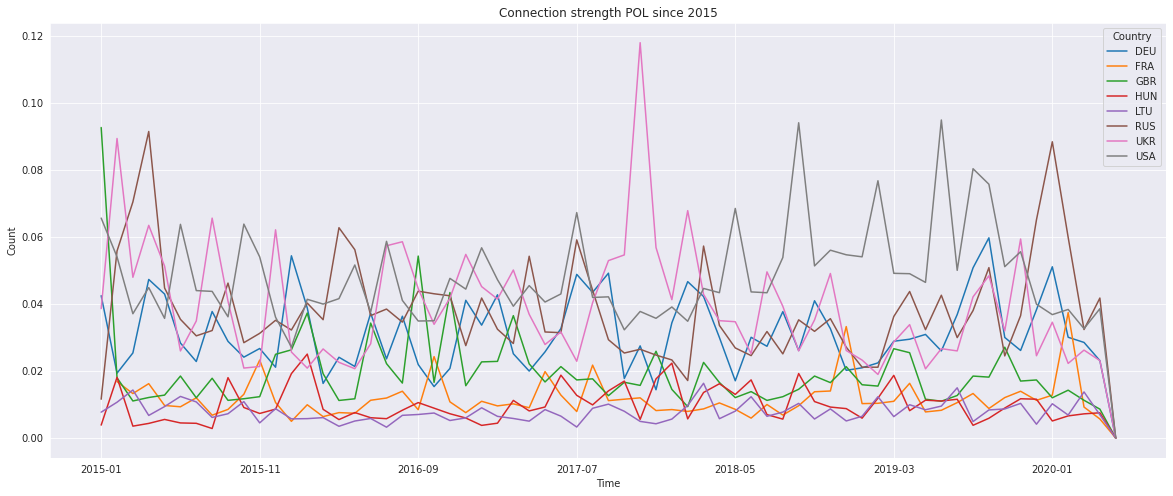
\includegraphics[width=\linewidth]{fig/PL/POLConnection.png}
        \caption{Siła połączenia Polski z wybranymi krajami w czasie. (źródło: opracowanie własne)}
        \label{fig:PLConnection}
    \end{figure}
    Pierwsza pozycja pod względem siły powiązania zmienia się w czasie.
    Od kwietnia 2018 do października 2019 zajmowały ją Stany Zjednoczone Ameryki.
    W pozostałym okresie obserwujemy największą siłę powiązania z Rosją oraz Ukrainą.

    \paragraph{Rosja}

    Wykres~\ref{fig:RUSConnection} przedstawia siłę połączenia Rosji z Niemcami oraz Polską w czasie
    \begin{figure}[!htp]
        \centering
        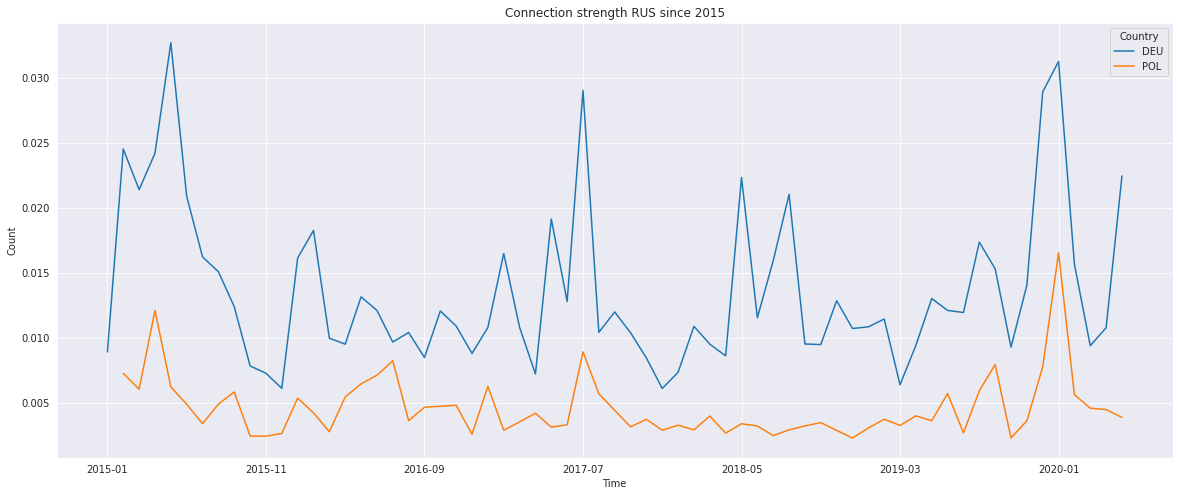
\includegraphics[width=\linewidth]{fig/RUS/RUSConnection.png}
        \caption{Siła połączenia Rosji z wybranymi krajami w czasie. (źródło: opracowanie własne)}
        \label{fig:RUSConnection}
    \end{figure}
    W całym analizowanym okresie siła połączenia między Rosją a Niemcami jest większa od siły połączenie Rosji z Polską.
    W czterech przypadkach obserwujemy wyraźną korelację wzrostu siły połączenia z Polską i z Niemcami.

    \paragraph{Niemcy}

    Wykres~\ref{fig:DEUConnection} przedstawia siłę połączenia Niemiec z wybranymi krajami w czasie.
    \begin{figure}[!htp]
        \centering
        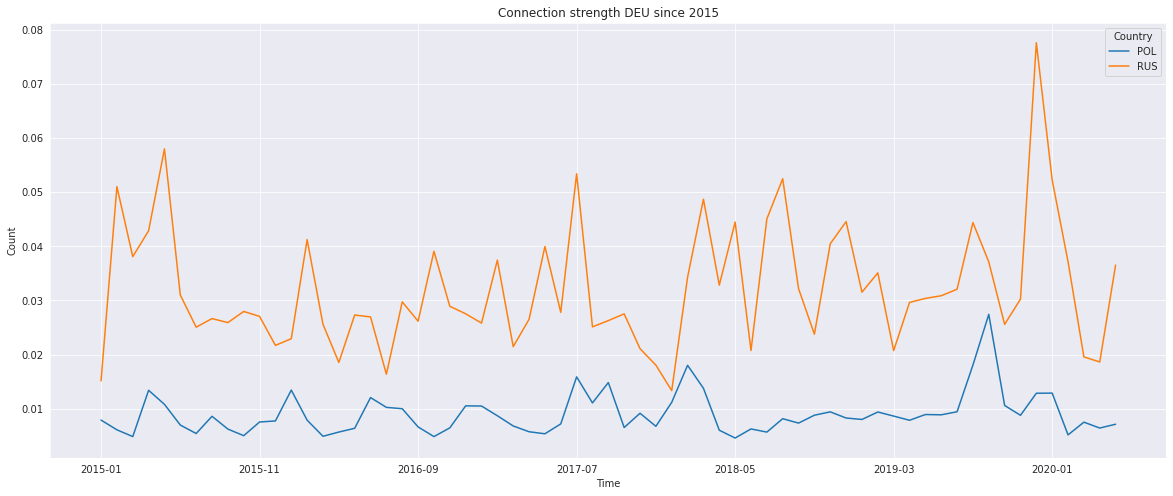
\includegraphics[width=\linewidth]{fig/DEU/DEUConnection.png}
        \caption{Siła połączenia Niemiec z wybranymi krajami w czasie. (źródło: opracowanie własne)}
        \label{fig:DEUConnection}
    \end{figure}
    Podobnie jak na wykresie~\ref{fig:RUSConnection} w całym analizowanym okresie siła połączenia z Polską jest mniejsza od siły połączenia z Rosją.

    \paragraph{Stany Zjednoczone}

    Wykres~\ref{fig:USAConnection} przedstawia siłę połączenia Stanów Zjednoczonych z wybranymi krajami w czasie.

    \begin{figure}[!htp]
        \centering
        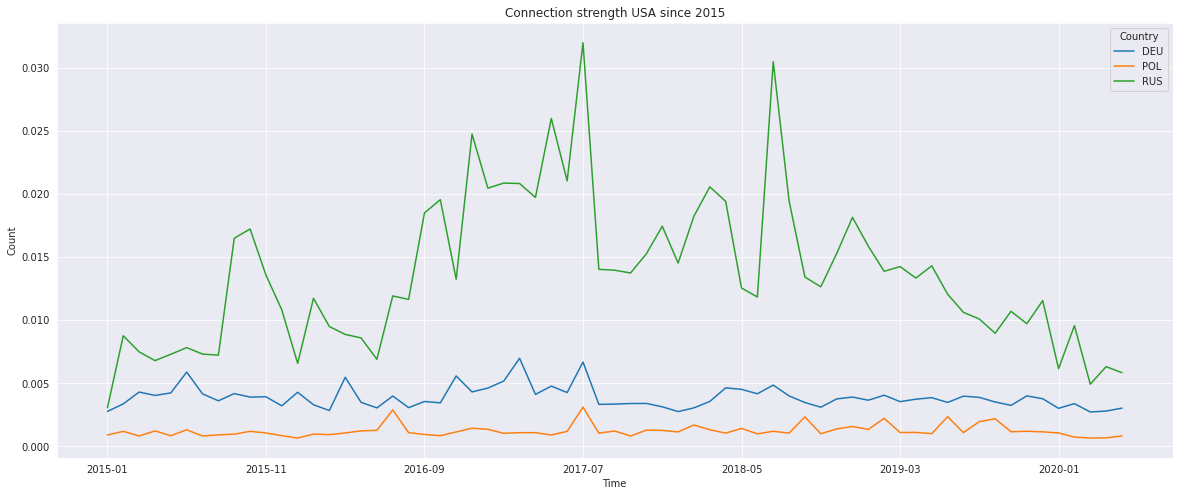
\includegraphics[width=\linewidth]{fig/USA/USAConnection.png}
        \caption{Siła połączenia Stanów Zjednoczonych z wybranymi krajami w czasie. (źródło: opracowanie własne)}
        \label{fig:USAConnection}
    \end{figure}
    Obserwujemy znacznie wyższą siłę połączenia Stanów Zjednoczonych z Rosją, niż z Niemcami oraz Polską.
    W lipcu 2017 obserwujemy korelację wzrostu siły połączenia Stanów Zjednoczonych z 3 analizowanymi krajami.
    W okresie od września 2017 do października 2018 obserwujemy zwiększoną siłę połączenia Stanów Zjednoczonych z Rosją.

    \subsection{Analiza symetryczności siły powiązania}

    \paragraph{Polska - Niemcy - Polska}

    Wykres~\ref{fig:POL-DEU-POL} przedstawia symetryczność siły połączenia Polski i~Niemiec w czasie.
    \begin{figure}[!htp]
        \centering
        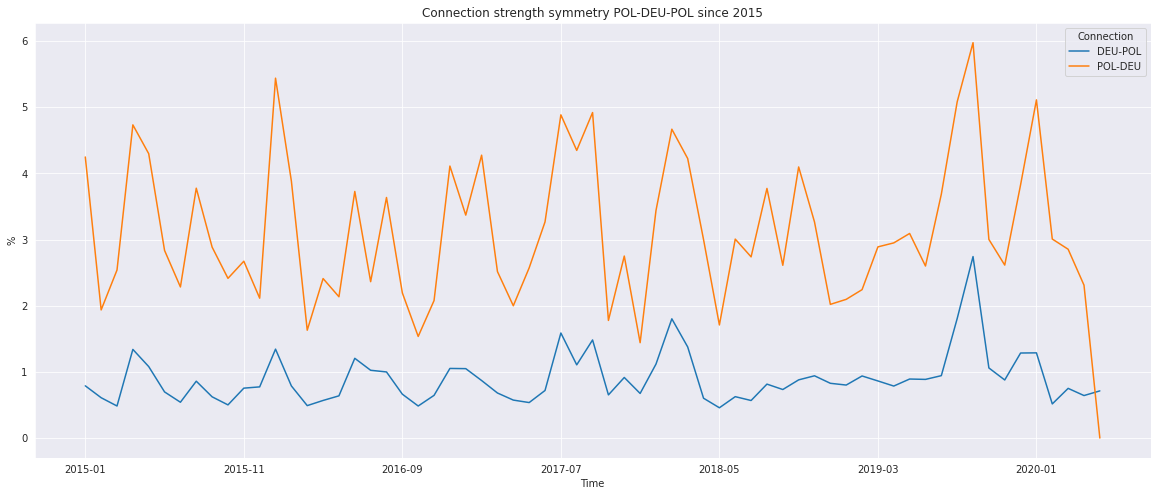
\includegraphics[width=\linewidth]{fig/ConnectionSymmetry/POL-DEU-POL.png}
        \caption{Symetryczność siły połączenia Polski i~Niemiec w czasie. (źródło: opracowanie własne)}
        \label{fig:POL-DEU-POL}
    \end{figure}
    Obserwujemy okresy korelacji siły połączenia Polski z Niemcami oraz Niemiec z Polską.
    W całym analizowanym okresie połączenie Polski z Niemcami jest silniejsze niż Niemiec z Polską.

    \paragraph{Polska - Rosja - Polska}

    Wykres~\ref{fig:POL-RUS-POL} przedstawia symetryczność siły połączenia Polski i~Rosji w czasie.
    \begin{figure}[!htp]
        \centering
        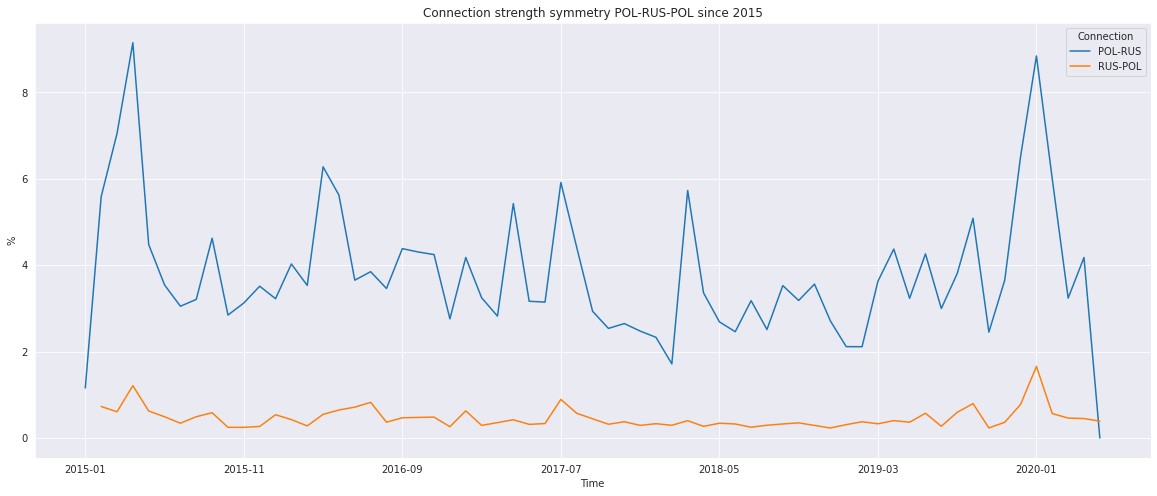
\includegraphics[width=\linewidth]{fig/ConnectionSymmetry/POL-RUS-POL.png}
        \caption{Symetryczność siły połączenia Polski i~Rosji w czasie. (źródło: opracowanie własne)}
        \label{fig:POL-RUS-POL}
    \end{figure}
    W porównaniu z wykresem~\ref{fig:POL-DEU-POL} obserwujemy słabsze połączenie Rosji z Polską niż Niemiec z Polską oraz silniejsze połączenie Polski z Rosją niż Polski z Niemcami.

    \paragraph{Polska - Stany Zjednoczone - Polska}

    Wykres~\ref{fig:POL-USA-POL} przedstawia symetryczność siły połączenia Polski i~Stanów Zjednoczonych w czasie.
    \begin{figure}[!htp]
        \centering
        \includegraphics[width=\linewidth]{fig/ConnectionSymmetry/POL-USA-POL.png}
        \caption{Symetryczność siły połączenia Polski i~Stanów Zjednoczonych w czasie. (źródło: opracowanie własne)}
        \label{fig:POL-USA-POL}
    \end{figure}
    Spośród analizowanych sił powiązania między Polską a Stanami Zjednoczonymi obserwujemy największą niesymetryczność relacji.
    Polska jest znacznie silniej powiązana ze Stanami Zjednoczonymi niż Stany Zjednoczone z Polską.
    Siła połączenia Stanów Zjednoczonych z Polską w całym analizowanym okresie utrzymuje się poniżej 0,5\%.


    \section{Analiza kodu podstawowego Fight}\label{sec:analiza-kodu-podstawowego-fight}

    Wykres~\ref{fig:Fight} przedstawia procentową liczbę państw z jakimi dany wybrany kraj ma zdarzenia fight w czasie.
    \begin{figure}[!htp]
        \centering
        \includegraphics[width=\linewidth]{fig/ERC/Fight.png}
        \caption{Procentowa liczba państw z jakimi dany wybrany kraj ma zdarzenia fight w czasie. (źródło: opracowanie własne)}
        \label{fig:Fight}
    \end{figure}
    Obserwujemy wystąpienie zdarzeń fight dla Polski mimo, iż nie prowadziła ona działań wojennych w tym okresie.
    Spowodowane jest to możliwością klasyfikowania do fight uroczystości mających na celu upamiętnienie wydarzeń historycznych.


    \chapter[Grupowanie państw]{Grupowanie państw o~podobnych cechach oraz~porównanie z danymi zewnętrznymi}\label{ch:grupowanie-państw-opodobnych-cechach-orazporównanie-z-danymi-zewnętrznymi}

    W tym rozdziale zostały opisane wyniki grupowania państw, z wykorzystaniem metody k-średnich, w oparciu o~podobne cechy z bazy danych GDELT.
    Dane zostały porównane z danymi zewnętrznymi.
    W części~\ref{sec:dane-niestandaryzowane} przedstawione zostały wyniki grupowania danych niestandaryzowanych.
    Część \ref{sec:dane-ustandaryzowane} zawiera wyniki grupowania danych ustandaryzowanych przy pomocy StandardScaler'a.
    Do grupowania krajów został wykorzystany wektor cech opisany w rozdziale~\ref{ch:koncepcja}.


    \section{Dane niestandaryzowane}\label{sec:dane-niestandaryzowane}
    W pierwszej kolejności zostaną przedstawione wyniki grupowania na danych niestandaryzowanych.

    Wykres~\ref{fig:clust10} przedstawia mapę z naniesionymi wynikami klasteryzacji.
    Każda grupa krajów otrzymała inny kolor.

    \begin{figure}[!htp]
        \centering
        \includegraphics[width=\linewidth]{fig/CLUST/10clusterMap.png}
        \caption{Mapa z wynikami klasteryzacji. (źródło: opracowanie własne)}
        \label{fig:clust10}
    \end{figure}

    Szczegółowe wyniki grupowania znajdują się w dodatku~\ref{ch:dodatek_niestd}.


    \section{Dane ustandaryzowane}\label{sec:dane-ustandaryzowane}
    Standrd Scaler standaryzuje cechy poprzez usunięcie średniej i~skalowanie do wariancji jednostkowej.
    Standardowy wynik próbki x jest obliczany jako:
    z = (x - u) / s
    gdzie u jest średnią próbek, a s jest standardowym odchyleniem próbek.

    Wykres~\ref{fig:clust10std} przedstawia mapę z naniesionymi wynikami klasteryzacji ustandaryzowanych próbek.
    Każda grupa krajów otrzymała inny kolor.

    \begin{figure}[!htp]
        \centering
        \includegraphics[width=\linewidth]{fig/CLUST/10clusterMap_std.png}
        \caption{Mapa z wynikami klasteryzacji. (źródło: opracowanie własne)}
        \label{fig:clust10std}
    \end{figure}

    Aby ułatwić interpretację wyników klasteryzacji poniżej dołączona została mapa~\ref{fig:clustPop} z naniesioną populacją oraz mapa~\ref{fig:clustGDP} z naniesionym PKB na osobę poszczególnych krajów, a także ich odpowiedniki ze skalą logarytmiczną~\ref{fig:clustPop_log} oraz~\ref{fig:clustGDP_log}.

    \begin{figure}[!htp]
        \centering
        \includegraphics[width=\linewidth]{fig/CLUST/population.png}
        \caption{Mapa z populacją krajów. (źródło: opracowanie własne)}
        \label{fig:clustPop}
    \end{figure}

    \begin{figure}[!htp]
        \centering
        \includegraphics[width=\linewidth]{fig/CLUST/gdp.png}
        \caption{Mapa z PKP na osobę. (źródło: opracowanie własne)}
        \label{fig:clustGDP}
    \end{figure}

    \begin{figure}[!htp]
        \centering
        \includegraphics[width=\linewidth]{fig/CLUST/population_log.png}
        \caption{Mapa z populacją krajów - skala logarytmiczna. (źródło: opracowanie własne)}
        \label{fig:clustPop_log}
    \end{figure}

    \begin{figure}[!htp]
        \centering
        \includegraphics[width=\linewidth]{fig/CLUST/gdp_log.png}
        \caption{Mapa z PKB na osobę - skala logarytmiczna. (źródło: opracowanie własne)}
        \label{fig:clustGDP_log}
    \end{figure}

    \begin{figure}[!htp]
        \centering
        \includegraphics[width=\linewidth]{fig/CLUST/gdp2015.png}
        \caption{Mapa z PKB - skala logarytmiczna. (źródło: opracowanie własne)}
        \label{fig:clustGDP2015_log}
    \end{figure}

    \begin{figure}[!htp]
        \centering
        \includegraphics[width=\linewidth]{fig/CLUST/health2015.png}
        \caption{Mapa z wydatkami na zdrowie - skala logarytmiczna. (źródło: opracowanie własne)}
        \label{fig:clustHealth2015_log}
    \end{figure}

    \begin{figure}[!htp]
        \centering
        \includegraphics[width=\linewidth]{fig/CLUST/military2015.png}
        \caption{Mapa z wydatkami na zbrojenia - skala logarytmiczna. (źródło: opracowanie własne)}
        \label{fig:clustMilitary2015_log}
    \end{figure}

    \begin{figure}[!htp]
        \centering
        \includegraphics[width=\linewidth]{fig/CLUST/import2015.png}
        \caption{Mapa z importem - skala logarytmiczna. (źródło: opracowanie własne)}
        \label{fig:clustImport2015_log}
    \end{figure}

    \begin{figure}[!htp]
        \centering
        \includegraphics[width=\linewidth]{fig/CLUST/export2015.png}
        \caption{Mapa z eksportem - skala logarytmiczna. (źródło: opracowanie własne)}
        \label{fig:clustExport2015_log}
    \end{figure}

    \subsection{Wyniki klasteryzacji - wykresy gęstości miar użytych do klastrowania - dane ustandaryzowane}
    Na wykresach od~\ref{fig:density_events} do~\ref{fig:density_expresscount} przedstawione zostały wykresy gęstości miar wykorzystanych przy grupowaniu w poszczególnych klastrach.

    \begin{figure}[!htp]
        \centering
        \includegraphics[width=\linewidth]{fig/CLUST/density_Events.png}
        \caption{Gęstość miary Events. (źródło: opracowanie własne)}
        \label{fig:density_events}
    \end{figure}

    Na wykresie~\ref{fig:density_events} obserwujemy słabą separację klastrów.
    Wyróżniają się klastry 7 oraz 8 których gęstości są spłaszczone i~wydłużone.

    \begin{figure}[!htp]
        \centering
        \includegraphics[width=\linewidth]{fig/CLUST/density_sumNumMentions.png}
        \caption{Gęstość miary sumNumMentions. (źródło: opracowanie własne)}
        \label{fig:density_sumnummentions}
    \end{figure}

    Na wykresie~\ref{fig:density_sumnummentions}, podobnie jak na poprzednim, obserwujemy słabą separację klastrów.
    Ponownie wyróżniają się klastry 7 oraz 8.

    \begin{figure}[!htp]
        \centering
        \includegraphics[width=\linewidth]{fig/CLUST/density_materialConfCoop.png}
        \caption{Gęstość miary materialConfCoop. (źródło: opracowanie własne)}
        \label{fig:density_materialconfcoop}
    \end{figure}

    Na wykresie~\ref{fig:density_materialconfcoop} obserwujemy dobrą separację klastrów 1, 3, 4, 5 oraz 8.

    \begin{figure}[!htp]
        \centering
        \includegraphics[width=\linewidth]{fig/CLUST/density_verbalConfCoop.png}
        \caption{Gęstość miary verbalConfCoop. (źródło: opracowanie własne)}
        \label{fig:density_verbalconfcoop}
    \end{figure}

    Na wykresie~\ref{fig:density_verbalconfcoop} zauważamy podobieństwo klastrów 1 i~9 oraz 3 i~7.

    \begin{figure}[!htp]
        \centering
        \includegraphics[width=\linewidth]{fig/CLUST/density_avgAvgTone.png}
        \caption{Gęstość miary avgAvgTone. (źródło: opracowanie własne)}
        \label{fig:density_avgavgtone}
    \end{figure}

    Na wykresie~\ref{fig:density_avgavgtone} wyróżnia się klaster 8 (największa gęstość) oraz klastry 7 i~8.


    \begin{figure}[!htp]
        \centering
        \includegraphics[width=\linewidth]{fig/CLUST/density_avgGoldstein.png}
        \caption{Gęstość miary avgGoldstein. (źródło: opracowanie własne)}
        \label{fig:density_avggoldstein}
    \end{figure}

    Na wykresie~\ref{fig:density_avggoldstein} najbardziej wyróżnia się klaster 8.
    Pozostałe (z wyjątkiem 2, 7 oraz 9) wyraźnie się oddzielają.

    \begin{figure}[!htp]
        \centering
        \includegraphics[width=\linewidth]{fig/CLUST/density_fightCount.png}
        \caption{Gęstość miary fightCount. (źródło: opracowanie własne)}
        \label{fig:density_fightcount}
    \end{figure}

    Na wykresie~\ref{fig:density_fightcount} większość klastrów osiąga maksimum gęstości w pobliżu wartości 0.

    \begin{figure}[!htp]
        \centering
        \includegraphics[width=\linewidth]{fig/CLUST/density_expressCount.png}
        \caption{Gęstość miary expressCount. (źródło: opracowanie własne)}
        \label{fig:density_expresscount}
    \end{figure}

    Na wykresie~\ref{fig:density_expresscount}, podobnie jak na poprzednim, obserwujemy skupienie w pobliżu zera.
    Wyróżniają się klastry 7 i~8, które są spłaszczone i~wydłużone.

    \subsection{Wyniki klasteryzacji w postaci tabelarycznej - dane ustandaryzowane}
    W tabelach od~\ref{tab:cl0std} do~\ref{tab:cl9std} przedstawione zostały wyniki grupowania ustandaryzowanych próbek.

    Zgodnie z założeniami z części~\ref{sec:założenia-i-wymagania}, dla ułatwienia interpretacji wyników grupowania, zostały dodane informacje zewnętrzne o~PKB i~wydatkach publicznych.
    Dodatkowo dokonano kolorowania pól z informacjami o~krajach.
    Poszczególne miary zostały podzielone na 5 równych przedziałów wg skali logarytmicznej.
    Kolory, od przedziału z najmniejszymi wartościami do tego z największymi, to: czerwony (bardzo niskie), pomarańczowy (niskie), żółty (średnie), jasnozielony (wysokie), zielony (bardzo wysokie).
    W tabelach od~\ref{tab:cl1stdcount} do~\ref{tab:cl9stdcount} została przedstawiona procentowa ilość państw w poszczególnych przedziałach w obrębie klastrów.
    W tabelach od~\ref{tab:cl0std_desc} do~\ref{tab:cl9std_desc} pokazane zostały parametry poszczególnych klastrów: średnia, mediana, odchylenie standardowe, minimum, maksimum.


    \begin{table}[!htp]
        \centering
        \includegraphics[width=\linewidth]{tables/CLUST/cluster0stdkmeans.png}
        \caption{Klaster 0 - dane standaryzowane. (źródło: opracowanie własne)}
        \label{tab:cl0std}
    \end{table}

    \begin{table}[!htp]
        \centering
        \includegraphics[width=\linewidth]{tables/CLUST/cluster0stdkmeanscount.png}
        \caption{Klaster 0 - ilość państw w poszczególnych przedziałach. (źródło: opracowanie własne)}
        \label{tab:cl0stdcount}
    \end{table}

    Klaster 0 w tabeli~\ref{tab:cl0std} zawiera 30 krajów.
    Przykłady ważniejszych państw w tym klastrze to: Estonia, Islandia, Luksemburg, Portugalia, Zjednoczone Emiraty Arabskie, Wietnam.
    W tabeli~\ref{tab:cl0stdcount} obserwujemy, że w klastrze 0 przeważają (2/3) kraje z niskimi i~średnimi wydatkami na opiekę zdrowotną (pomiędzy 3, a 7.9\% PKB).

    \begin{table}[!htp]
        \centering
        \includegraphics[width=\linewidth]{tables/CLUST/desc/clust0std_desc.png}
        \caption{Parametry klastra 0 - dane standaryzowane. (źródło: opracowanie własne)}
        \label{tab:cl0std_desc}
    \end{table}

    \begin{table}[!htp]
        \centering
        \includegraphics[width=\linewidth]{tables/CLUST/cluster1stdkmeans.png}
        \caption{Klaster 1 - dane standaryzowane. (źródło: opracowanie własne)}
        \label{tab:cl1std}
    \end{table}

    \begin{table}[!htp]
        \centering
        \includegraphics[width=\linewidth]{tables/CLUST/cluster1stdkmeanscount.png}
        \caption{Klaster 1 - ilość państw w poszczególnych przedziałach. (źródło: opracowanie własne)}
        \label{tab:cl1stdcount}
    \end{table}

    Klaster 1 w tabeli~\ref{tab:cl1std} zawiera 3 kraje - Indie, Liban oraz Palestynę.
    W tabeli~\ref{tab:cl1stdcount} obserwujemy, że wszystkie państwa w klastrze 1 charakteryzują się średnim eksportem (pomiędzy 2.5\%, a 5.1\% PKB).

    \begin{table}[!htp]
        \centering
        \caption{Parametry klastra 1 - dane standaryzowane. (źródło: opracowanie własne)}
        \label{tab:cl1std_desc}
        \includegraphics[width=\linewidth]{tables/CLUST/desc/clust1std_desc.png}
    \end{table}

    \begin{table}[!htp]
        \centering
        \includegraphics[width=\linewidth]{tables/CLUST/cluster2stdkmeans.png}
        \caption{Klaster 2 - dane standaryzowane. (źródło: opracowanie własne)}
        \label{tab:cl2std}
    \end{table}

    \begin{table}[!htp]
        \centering
        \includegraphics[width=\linewidth]{tables/CLUST/cluster2stdkmeanscount.png}
        \caption{Klaster 2 - ilość państw w poszczególnych przedziałach. (źródło: opracowanie własne)}
        \label{tab:cl2stdcount}
    \end{table}

    Klaster 2 w tabeli~\ref{tab:cl2std} zawiera 3 kraje - Botswanę, Gwineę Bissau oraz .
    W tabeli~\ref{tab:cl2stdcount} obserwujemy, że wszystkie państwa w klastrze 2 charakteryzują się niskim eksportem (pomiędzy 1.2\%, a 2.5\% PKB).

    \begin{table}[!htp]
        \centering
        \includegraphics[width=\linewidth]{tables/CLUST/desc/clust2std_desc.png}
        \caption{Parametry klastra 2 - dane standaryzowane. (źródło: opracowanie własne)}
        \label{tab:cl2std_desc}
    \end{table}

    \begin{table}[!htp]
        \centering
        \includegraphics[width=\linewidth]{tables/CLUST/cluster3stdkmeans.png}
        \caption{Klaster 3 - dane standaryzowane. (źródło: opracowanie własne)}
        \label{tab:cl3std}
    \end{table}

    \begin{table}[!htp]
        \centering
        \includegraphics[width=\linewidth]{tables/CLUST/desc/clust3std_desc.png}
        \caption{Parametry klastra 3 - dane standaryzowane. (źródło: opracowanie własne)}
        \label{tab:cl3std_desc}
    \end{table}

    \begin{table}[!htp]
        \centering
        \includegraphics[width=\linewidth]{tables/CLUST/cluster3stdkmeanscount.png}
        \caption{Klaster 3 - ilość państw w poszczególnych przedziałach. (źródło: opracowanie własne)}
        \label{tab:cl3stdcount}
    \end{table}

    Klaster 3 w tabeli~\ref{tab:cl3std} zwiera 10 krajów.
    Przykłady ważniejszych państw w tym klastrze to: Chiny, Francja, Niemcy, Rosja, Wielka Brytania.
    W tabeli~\ref{tab:cl3stdcount} obserwujemy, że w klastrze 3 przeważają kraje z wysokim oraz bardzo wysokim PKB (pomiędzy 3.23e+11\$, a 1.82e+13\$).

    \begin{table}[!htp]
        \centering
        \includegraphics[width=\linewidth]{tables/CLUST/cluster4stdkmeans.png}
        \caption{Klaster 4 - dane standaryzowane. (źródło: opracowanie własne)}
        \label{tab:cl4std}
    \end{table}

    \begin{table}[!htp]
        \centering
        \includegraphics[width=\linewidth]{tables/CLUST/cluster4stdkmeanscount.png}
        \caption{Klaster 4 - ilość państw w poszczególnych przedziałach. (źródło: opracowanie własne)}
        \label{tab:cl4stdcount}
    \end{table}

    Klaster 4 w tabeli~\ref{tab:cl4std} zawiera 8 krajów.
    Przykłady ważniejszych państw w tym klastrze to: Kenia, Somalia, Syria.
    W tabeli~\ref{tab:cl4stdcount} obserwujemy, że w klastrze 4 przeważają kraje z niskim PKB (pomiędzy 5.71e+09\$, a 4.29e+10\$).

    \begin{table}[!htp]
        \centering
        \includegraphics[width=\linewidth]{tables/CLUST/desc/clust4std_desc.png}
        \caption{Parametry klastra 4 - dane standaryzowane. (źródło: opracowanie własne)}
        \label{tab:cl4std_desc}
    \end{table}

    \begin{table}[!htp]
        \centering
        \includegraphics[width=\linewidth]{tables/CLUST/cluster5stdkmeans.png}
        \caption{Klaster 5 - dane standaryzowane. (źródło: opracowanie własne)}
        \label{tab:cl5std}
    \end{table}

    \begin{table}[!htp]
        \centering
        \includegraphics[width=\linewidth]{tables/CLUST/cluster5stdkmeanscount.png}
        \caption{Klaster 5 - ilość państw w poszczególnych przedziałach. (źródło: opracowanie własne)}
        \label{tab:cl5stdcount}
    \end{table}

    Klaster 5 w tabeli~\ref{tab:cl5std} zawiera 21 krajów.
    Przykłady ważniejszych państw w tym klastrze to: Chile, Nigeria, Pakistan, Polska, Szwecja.
    W tabeli~\ref{tab:cl5stdcount} obserwujemy, że w klastrze 5 przeważają kraje ze średnimi wydatkami na opiekę zdrowotną (pomiędzy 4.9\%, a 7.9\% PKB).

    \begin{table}[!htp]
        \centering
        \includegraphics[width=\linewidth]{tables/CLUST/desc/clust5std_desc.png}
        \caption{Parametry klastra 5 - dane standaryzowane. (źródło: opracowanie własne)}
        \label{tab:cl5std_desc}
    \end{table}

    \begin{table}[!htp]
        \centering
        \includegraphics[width=\linewidth]{tables/CLUST/cluster6stdkmeans.png}
        \caption{Klaster 6 - dane standaryzowane. (źródło: opracowanie własne)}
        \label{tab:cl6std}
    \end{table}

    \begin{table}[!htp]
        \centering
        \includegraphics[width=\linewidth]{tables/CLUST/cluster6stdkmeanscount.png}
        \caption{Klaster 6 - ilość państw w poszczególnych przedziałach. (źródło: opracowanie własne)}
        \label{tab:cl6stdcount}
    \end{table}

    Klaster 6 w tabeli~\ref{tab:cl6std} zawiera 49 krajów.
    Przykłady ważniejszych państw w tym klastrze to: Białoruś, Bułgaria, Czechy, Finlandia, Węgry, Norwegia.
    W tabeli~\ref{tab:cl6stdcount} obserwujemy, że w klastrze 6 przeważają kraje z wysokimi wydatkami na edukację (pomiędzy 4\%, a 5.5\% PKB).

    \begin{table}[!htp]
        \centering
        \includegraphics[width=\linewidth]{tables/CLUST/desc/clust6std_desc.png}
        \caption{Parametry klastra 6 - dane standaryzowane. (źródło: opracowanie własne)}
        \label{tab:cl6std_desc}
    \end{table}

    \begin{table}[!htp]
        \centering
        \includegraphics[width=\linewidth]{tables/CLUST/cluster7stdkmeans.png}
        \caption{Klaster 7 - dane standaryzowane. (źródło: opracowanie własne)}
        \label{tab:cl7std}
    \end{table}

    \begin{table}[!htp]
        \centering
        \includegraphics[width=\linewidth]{tables/CLUST/cluster7stdkmeanscount.png}
        \caption{Klaster 7 - ilość państw w poszczególnych przedziałach. (źródło: opracowanie własne)}
        \label{tab:cl7stdcount}
    \end{table}

    Klaster 7 w tabeli~\ref{tab:cl7std} zawiera 2 kraje - Iran i~Irak.
    W tabeli~\ref{tab:cl7stdcount} obserwujemy, że w klastrze 7 żaden z parametrów nie wyróżnia się.

    \begin{table}[!htp]
        \centering
        \includegraphics[width=\linewidth]{tables/CLUST/desc/clust7std_desc.png}
        \caption{Parametry klastra 7 - dane standaryzowane}
        \label{tab:cl7std_desc}
    \end{table}

    \begin{table}[!htp]
        \centering
        \includegraphics[width=\linewidth]{tables/CLUST/cluster8stdkmeans.png}
        \caption{Klaster 8 - dane standaryzowane. (źródło: opracowanie własne)}
        \label{tab:cl8std}
    \end{table}

    \begin{table}[!htp]
        \centering
        \includegraphics[width=\linewidth]{tables/CLUST/cluster8stdkmeanscount.png}
        \caption{Klaster 8 - ilość państw w poszczególnych przedziałach. (źródło: opracowanie własne)}
        \label{tab:cl8stdcount}
    \end{table}

    Klaster 8 w tabeli~\ref{tab:cl8std} posiada tylko jedno państwo - Stany Zjednoczone Ameryki.
    W tabeli~\ref{tab:cl8stdcount} obserwujemy, że klaster 8 wyróżnia sie bardzo wysokim PKB (2.42e+12\$, a 1.82e+13\$).

    \begin{table}[!htp]
        \centering
        \includegraphics[width=\linewidth]{tables/CLUST/desc/clust8std_desc.png}
        \caption{Parametry klastra 8 - dane standaryzowane. (źródło: opracowanie własne)}
        \label{tab:cl8std_desc}
    \end{table}

    \begin{table}[!htp]
        \centering
        \includegraphics[width=\linewidth]{tables/CLUST/cluster9stdkmeans.png}
        \caption{Klaster 9 - dane standaryzowane. (źródło: opracowanie własne)}
        \label{tab:cl9std}
    \end{table}

    \begin{table}[!htp]
        \centering
        \includegraphics[width=\linewidth]{tables/CLUST/cluster9stdkmeanscount.png}
        \caption{Klaster 9 - ilość państw w poszczególnych przedziałach. (źródło: opracowanie własne)}
        \label{tab:cl9stdcount}
    \end{table}

    Klaster 9 w tabeli~\ref{tab:cl9std} zawiera 31 krajów.
    Przykłady ważniejszych państw w tym klastrze to: Gwatemala, Honduras, Kuwejt, Meksyk, Słowacja.
    W tabeli~\ref{tab:cl9stdcount} obserwujemy, że klaster 9 wyróżnia sie niskimi wydatkami na zbrojenia (pomiędzy 0.7\%, a 1.48\% PKB).

    \begin{table}[!htp]
        \centering
        \includegraphics[width=\linewidth]{tables/CLUST/desc/clust9std_desc.png}
        \caption{Parametry klastra 9 - dane standaryzowane. (źródło: opracowanie własne)}
        \label{tab:cl9std_desc}
    \end{table}

    Tabele~\ref{tab:cl_mean_summ} oraz~\ref{tab:cl_median_summ} zawierają podsumowanie parametrów poszczególnych klastrów.

    \begin{table}[!htp]
        \centering
        \includegraphics[width=\linewidth]{tables/CLUST/desc/cluster_mean_summary.png}
        \caption{Średnie wartości parametrów w klastrach. (źródło: opracowanie własne)}
        \label{tab:cl_mean_summ}
    \end{table}

    W tabeli~\ref{tab:cl_mean_summ} wyraźnie oddziela się klaster 8 - hegemon, Stany Zjednoczone Ameryki - bardzo wysokie PKB, wydatki na zdrowie, wysokie wydatki na zbrojenia, niski import.
    Kolejnym wyróżniają się klastrem jest klaster 7 - Irak i~Iran - najwyższe średni wydatki na zbrojenia.
    Klaster 3 - kraje bogate - wysokie PKB i~wydatki na opiekę
    Klaster 4 - ubogie kraje afrykańskie i~bliskiego wschodu - niskie PKB.

    \begin{table}[!htp]
        \centering
        \includegraphics[width=\linewidth]{tables/CLUST/desc/cluster_median_summary.png}
        \caption{Mediany wartości parametrów w klastrach. (źródło: opracowanie własne)}
        \label{tab:cl_median_summ}
    \end{table}


    Zarówno dla danych nie poddanych oraz poddanych standaryzacji Stany Zjednoczono otrzymały własny klaster.
    Jest to spowodowane znaczącą przewagą liczby zdarzeń w porównaniu z innymi krajami.

    Dla danych standaryzowanych Polska i~Szwecja są jedynymi krajami europejskim w klastrze~\ref{tab:cl5std}.


    \chapter{Podsumowanie}\label{ch:podsumowanie}
    W niniejszym rozdziale w części~\ref{sec:wnioski} zostaną opisane wnioski z pracy według kolejności wcześniej przedstawionych rozdziałów.
    W części~\ref{sec:dalsze-kierunki-rozwoju} zawarto propozycje dalszych kierunków rozwoju.


    \section{Wnioski}\label{sec:wnioski}
    Przeprowadzona analiza danych ze zbioru GDELT pozwoliła na wybranie takiego wektora cech który umożliwił skuteczny podział państw - aktorów - na grupy.
    Udało się wykazać związek powstałych klastrów z rzeczywistymi cechami państw.
    Najwyraźniejszymi


    \section{Dalsze kierunki rozwoju}\label{sec:dalsze-kierunki-rozwoju}
    Poniżej przedstawiono propozycje dalszych kierunków rozwoju pracy.

    \paragraph{Badanie innych wektorów grupowania}
    Próba znalezienia cech zdarzeń lepiej odpowiadających rzeczywistym podziałom krajów na grupy.

    \paragraph{Analiza dynamiczna grupowania krajów}
    Przeprowadzenie klasteryzacji w kolejnych przedziałach czasowych.
    Analiza zmian przynależności krajów do klastrów.

    \paragraph{Analiza pod kątem COVID-19}
    Analiza danych z bazy GDELT pod kątem zmian w relacjach krajów spowodowanych rozwojem pandemii koronawirusa.
    Sprawdzenie czy wzorce zmian zachowań obserwowanych podczas pandemii występowały już wcześniej.

    \paragraph{Analiza pod kątem grup etnicznych}
    Analiza zdarzeń z podziałem na grupy etniczne.
    Klastrowanie grup etnicznych.

    \paragraph{Analiza pod kątem grup religijnych}
    Analiza zdarzeń z podziałem na grupy religijne.
    Klastrowanie grup religijnych.

    \appendix
    \newpage


    \chapter[Wyniki grupowania]{Wyniki grupowania danych niestandaryzowanych}\label{ch:dodatek_niestd}
    W tym dodatku przedstawione zostały wyniki klasteryzacji danych nie poddanych standaryzacji.

    W tabelach od~\ref{tab:cl0} do~\ref{tab:cl9} przedstawione zostały wyniki grupowania.
    Dodatkowo zawarto informacje o~liczbie ludności i~PKB na osobę pochodzące z biblioteki GeoPandas~\cite{geopandas}.

    Klaster 0 w tabeli~\ref{tab:cl0} zawiera 4 kraje.
    \begin{table}[!htp]
        \centering
        \includegraphics[width=\linewidth]{tables/CLUST/clust0kmeans.png}
        \caption{Klaster 0. (źródło: opracowanie własne)}
        \label{tab:cl0}
    \end{table}

    Klaster 1 w tabeli~\ref{tab:cl1} zawiera 15 krajów.
    \begin{table}[!htp]
        \centering
        \includegraphics[width=\linewidth]{tables/CLUST/clust1kmeans.png}
        \caption{Klaster 1. (źródło: opracowanie własne)}
        \label{tab:cl1}
    \end{table}

    Klaster 2 w tabeli~\ref{tab:cl2} zawiera 34 kraje.
    \begin{table}[!htp]
        \centering
        \includegraphics[width=\linewidth]{tables/CLUST/clust2kmeans.png}
        \caption{Klaster 2. (źródło: opracowanie własne)}
        \label{tab:cl2}
    \end{table}

    Klaster 3 w tabeli~\ref{tab:cl3} zawiera 8 krajów.
    \begin{table}[!htp]
        \centering
        \includegraphics[width=\linewidth]{tables/CLUST/clust3kmeans.png}
        \caption{Klaster 3. (źródło: opracowanie własne)}
        \label{tab:cl3}
    \end{table}

    Klaster 4 w tabeli~\ref{tab:cl4} zawiera 31 krajów.
    \begin{table}[!htp]
        \centering
        \includegraphics[width=\linewidth]{tables/CLUST/clust4kmeans.png}
        \caption{Klaster 4. (źródło: opracowanie własne)}
        \label{tab:cl4}
    \end{table}

    Klaster 5 w tabeli~\ref{tab:cl5} zawiera 13 krajów.
    \begin{table}[!htp]
        \centering
        \includegraphics[width=\linewidth]{tables/CLUST/clust5kmeans.png}
        \caption{Klaster 5. (źródło: opracowanie własne)}
        \label{tab:cl5}
    \end{table}

    Klaster 6 w tabeli~\ref{tab:cl6} zawiera 35 krajów.
    \begin{table}[!htp]
        \centering
        \includegraphics[width=\linewidth]{tables/CLUST/clust6kmeans.png}
        \caption{Klaster 6. (źródło: opracowanie własne)}
        \label{tab:cl6}
    \end{table}

    Klaster 7 w tabeli~\ref{tab:cl7} zawiera 9 krajów.
    \begin{table}[!htp]
        \centering
        \includegraphics[width=\linewidth]{tables/CLUST/clust7kmeans.png}
        \caption{Klaster 7. (źródło: opracowanie własne)}
        \label{tab:cl7}
    \end{table}

    Klaster 8 w tabeli~\ref{tab:cl8} zawiera tylko jeden kraj - Stany Zjednoczone Ameryki.
    \begin{table}[!htp]
        \centering
        \includegraphics[width=\linewidth]{tables/CLUST/clust8kmeans.png}
        \caption{Klaster 8. (źródło: opracowanie własne)}
        \label{tab:cl8}
    \end{table}

    Klaster 9 w tabeli~\ref{tab:cl9} zawiera 12 krajów.
    \begin{table}[!htp]
        \centering
        \includegraphics[width=\linewidth]{tables/CLUST/clust9kmeans.png}
        \caption{Klaster 9. (źródło: opracowanie własne)}
        \label{tab:cl9}
    \end{table}

    Dla danych niestandaryzowanych Polska trafiła do klastra~\ref{tab:cl9} między innymi z Egiptem, Grecją, Irlandia oraz Brazylią.
    Wyróżnia się mniejsza grupa~\ref{tab:cl0} do której trafiły Chiny, Rosja, Wielka Brytania oraz Iran.

    \inputencoding{utf8}

    \newpage
    \addcontentsline{toc}{chapter}{Bibliografia}
    \printbibliography[title={Bibliografia}]

\end{document}
